%
% Template per Elaborato di Laurea
% DISI - Dipartimento di Ingegneria e Scienza dell’Informazione
%
% update 2015-09-10
%
% Per la generazione corretta del 
% pdflatex nome_file.tex
% bibtex nome_file.aux
% pdflatex nome_file.tex
% pdflatex nome_file.tex
%
%%%%%%%%%%%%%%%%%%%%%%%%%%%%%%%%%%%%%%%%%%%%%%%

% formato FRONTE RETRO
\documentclass[epsfig,a4paper,11pt,titlepage,twoside,openany]{book}
\usepackage{epsfig}
\usepackage{plain}
\usepackage{setspace}
\usepackage{graphicx}
\usepackage{caption}
\usepackage{subcaption}
\usepackage{cleveref}
\usepackage{wrapfig}
\usepackage{xcolor}
\usepackage[paperheight=29.7cm,paperwidth=21cm,outer=1.5cm,inner=2.5cm,top=2cm,bottom=2cm]{geometry} % per definizione layout
\usepackage{titlesec} % per formato custom dei titoli dei capitoli
\graphicspath{ {./images/} }

%%%%%%%%%%%%%%
% supporto lettere accentate
%
%\usepackage[latin1]{inputenc} % per Windows;
\usepackage[utf8x]{inputenc} % per Linux (richiede il pacchetto unicode);
%\usepackage[applemac]{inputenc} % per Mac.

\singlespacing

\usepackage[italian]{babel}

\begin{document}

  % nessuna numerazione
  \pagenumbering{gobble} 
  
    % Declare new goemetry for the title page only.
    \newgeometry{outer=2cm,inner=2cm,top=2cm,bottom=2cm}
    %---------------------------------------------
    \pagestyle{plain}

\thispagestyle{empty}

\begin{center}
    \begin{figure}[h!]
        \centerline{\includegraphics[width=0.6\textwidth]{marchio_unitrento_colore_it_202002.eps}}
    \end{figure}
    \vspace{1 cm}

    \LARGE{Dipartimento di Ingegneria e Scienza dell'Informazione\\}

    \vspace{2 cm}
    \Large{Corso di Laurea in\\
    Informatica
    %Ingegneria dell'Informazione e delle Comunicazioni
    %Ingegneria dell'Informazione e Organizzazione d'Impresa
    %Ingegneria Elettronica e delle Telecomunicazioni
    }

    \vspace{2 cm}
    \Large\textsc{Elaborato finale\\}
    \vspace{1 cm}
    \Huge\textsc{VolleyVisionAI: Web App per l'Analisi Video nella Pallavolo\\}

    \vspace{2 cm}
    \begin{tabular*}{\textwidth}{ c @{\extracolsep{\fill}} c }
    \Large{Supervisore} & \Large{Laureando}\\
    \Large{Luca Turchet} & \Large{Andrea Richichi}\\
    \\
    \Large{Co-supervisore} & \\
    \Large{Maurizio Napolitano} & \\
    \end{tabular*}

    \vspace{2 cm}

    \Large{Anno accademico 2023/2024}

\end{center}

    % Ends the declared geometry for the titlepage
    \restoregeometry
    %--------------------------


  \newpage
  
  
%%%%%%%%%%%%%%%%%%%%%%%%%%%%%%%%%%%%%%%%%%%%%%%%%%%%%%%%%%%%%%%%%%%%%%%%%%
%%%%%%%%%%%%%%%%%%%%%%%%%%%%%%%%%%%%%%%%%%%%%%%%%%%%%%%%%%%%%%%%%%%%%%%%%%
%% Nota
%%%%%%%%%%%%%%%%%%%%%%%%%%%%%%%%%%%%%%%%%%%%%%%%%%%%%%%%%%%%%%%%%%%%%%%%%%
%% Sezione Ringraziamenti opzionale
%%%%%%%%%%%%%%%%%%%%%%%%%%%%%%%%%%%%%%%%%%%%%%%%%%%%%%%%%%%%%%%%%%%%%%%%%%
%%%%%%%%%%%%%%%%%%%%%%%%%%%%%%%%%%%%%%%%%%%%%%%%%%%%%%%%%%%%%%%%%%%%%%%%%%
  \input{ringraziamenti}
  \pagestyle{plain} % nessuna intestazione e pie pagina con numero al centro
    
  
  % inizio numerazione pagine in numeri arabi
  \mainmatter

%%%%%%%%%%%%%%%%%%%%%%%%%%%%%%%%%%%%%%%%%%%%%%%%%%%%%%%%%%%%%%%%%%%%%%%%%%
%%%%%%%%%%%%%%%%%%%%%%%%%%%%%%%%%%%%%%%%%%%%%%%%%%%%%%%%%%%%%%%%%%%%%%%%%%
%% Nota
%%%%%%%%%%%%%%%%%%%%%%%%%%%%%%%%%%%%%%%%%%%%%%%%%%%%%%%%%%%%%%%%%%%%%%%%%%
%% Si ricorda che il numero massimo di facciate e' 30.
%% Nel conteggio delle facciate sono incluse 
%%   indice
%%   sommario
%%   capitoli
%% Dal conteggio delle facciate sono escluse
%%   frontespizio
%%   ringraziamenti
%%   allegati    
%%%%%%%%%%%%%%%%%%%%%%%%%%%%%%%%%%%%%%%%%%%%%%%%%%%%%%%%%%%%%%%%%%%%%%%%%%
%%%%%%%%%%%%%%%%%%%%%%%%%%%%%%%%%%%%%%%%%%%%%%%%%%%%%%%%%%%%%%%%%%%%%%%%%%

    % indice
    \tableofcontents
    \clearpage
    
    
          
    % gruppo per definizone di successione capitoli senza interruzione di pagina
    \begingroup
      % nessuna interruzione di pagina tra capitoli
      % ridefinizione dei comandi di clear page
      \renewcommand{\cleardoublepage}{} 
      \renewcommand{\clearpage}{} 
      % redefinizione del formato del titolo del capitolo
      % da formato
      %   Capitolo X
      %   Titolo capitolo
      % a formato
      %   X   Titolo capitolo
      
      \titleformat{\chapter}
        {\normalfont\Huge\bfseries}{\thechapter}{1em}{}
        
      \titlespacing*{\chapter}{0pt}{0.59in}{0.02in}
      \titlespacing*{\section}{0pt}{0.20in}{0.02in}
      \titlespacing*{\subsection}{0pt}{0.10in}{0.02in}
      
      % sommario
      \chapter*{Abstract}
\label{Abstract}
\addcontentsline{toc}{chapter}{Abstract}

L'elaborato presenta lo sviluppo e l'implementazione di \textit{VolleyVisionAI}, una Web App progettata per l'analisi video nello sport della pallavolo. L'obiettivo principale è quello di colmare il vuoto di mercato tra gli strumenti professionali, spesso inaccessibili, e l'esigenza di un'applicazione intuitiva e semplice rivolta ad un'utenza amatoriale. 

\textit{VolleyVisionAI} presenta due modalità di funzionamento: la modalità manuale, che permette agli utenti di creare, importare ed esportare progetti di analisi video, effettuare \textit{Event Tagging} e generare videoclip personalizzati; e la modalità AI, che utilizza modelli di \textit{Computer Vision} per tracciare la palla e riconoscere i giocatori in campo. Queste funzionalità sono state implementate sviluppando un'architettura che garantisce alte prestazioni e scalabilità, con \textit{React.js} per il front-end e \textit{FastAPI} per il back-end.

Il processo di sviluppo ha compreso l'analisi dei requisiti, la creazione di un prototipo iniziale con \textit{Figma}, e lo sviluppo tecnico di interfaccia utente in \textit{JavaScript} e funzionalità back-end in \textit{Python}. Queste ultime comprendono l'analisi tramite AI per la quale è stato integrato il modello di riconoscimento \textit{YOLOv9} e la libreria \textit{OpenCV}. 

I test di usabilità effettuati hanno confermato l'efficacia dell'applicazione e l'intuitività della sua interfaccia. Inoltre i feedback ricevuti hanno permesso di migliorare ulteriormente la \textit{user-experience} e offrire spunti per sviluppi futuri dell'app. 
La versione beta di \textit{VolleyVisionAI} è attualmente operativa e ha raggiunto pienamente gli obiettivi prefissati. I risultati ottenuti offrono nuove opportunità per il futuro, tra cui l'aggiunta di nuove funzionalità nella modalità AI e l'estensione dell'accessibilità attraverso un sistema di \textit{Deployment}.

%%%%%%%%%%%%%%%%%%%%%%%%%%%%%%%%%%%%%%%%%%%%%%%%%%%%%%%%%%%%%%%%%%%%%%%%%%
%%%%%%%%%%%%%%%%%%%%%%%%%%%%%%%%%%%%%%%%%%%%%%%%%%%%%%%%%%%%%%%%%%%%%%%%%%
%% Nota
%%%%%%%%%%%%%%%%%%%%%%%%%%%%%%%%%%%%%%%%%%%%%%%%%%%%%%%%%%%%%%%%%%%%%%%%%%
%% Sommario e' un breve riassunto del lavoro svolto dove si descrive 
%% l’obiettivo, l’oggetto della tesi, le metodologie e 
%% le tecniche usate, i dati elaborati e la spiegazione delle conclusioni 
%% alle quali siete arrivati.
%% Il sommario dell’elaborato consiste al massimo di 3 pagine e deve contenere le seguenti informazioni: 
%%   contesto e motivazioni+
%%   breve riassunto del problema affrontato
%%   tecniche utilizzate e/o sviluppate
%%   risultati raggiunti, sottolineando il contributo personale del laureando/a
%%%%%%%%%%%%%%%%%%%%%%%%%%%%%%%%%%%%%%%%%%%%%%%%%%%%%%%%%%%%%%%%%%%%%%%%%%
%%%%%%%%%%%%%%%%%%%%%%%%%%%%%%%%%%%%%%%%%%%%%%%%%%%%%%%%%%%%%%%%%%%%%%%%%%      
      
      %%%%%%%%%%%%%%%%%%%%%%%%%%%%%%%%
      % lista dei capitoli
      %
      % \input oppure \include
      %
      \newpage
      \chapter{Introduzione}
\label{cha:introduzione}


L'obiettivo di questo progetto è sviluppare una Web App per l'analisi video nel volley dedicata ad allenatori e atleti. L'idea nasce in seguito ad alcune ricerche di mercato che hanno evidenziato l'assenza di soluzioni \textit{user-friendly} gratuite, per l'analisi video nello sport della pallavolo, adatte ad utenti amatoriali. L'applicazione, rispetto ad altre soluzioni già presenti sul mercato, ha infatti lo scopo principale di avere una \textit{User Interface} estremamente semplice ed intuitiva, offrendo allo stesso tempo un riuso gratuito. Questo permette di garantire una \textit{User Experience} di alto livello, qualunque siano le conoscenze tecniche dell'utente finale.

Le competenze accademiche e lavorative acquisite durante il percorso di laurea Triennale in Informatica a Trento, sono risultate fondamentali in fase di progettazione e sviluppo. Il corso online tenuto da EyeStudios Academy \cite{EyeStudios-Academy} su \textit{Figma} ha fornito l'esperienza necessaria per realizzare un prototipo interattivo dell'app, velocizzando così il processo di sviluppo.

L'esperienza di tirocinio presso la \textit{Fondazione Bruno Kessler} ha inoltre contribuito a consolidare la conoscenza della libreria \textit{React} e del linguaggio \textit{JavaScript}, ampiamente utilizzati nello lo sviluppo della Web App.

Il corso di Ingegneria del Software ha aiutato a definire, in fase di analisi e progettazione, le funzionalità dell'app individuando requisiti funzionali e non funzionali.

Il resto dell'elaborato prevede questi capitoli:

\begin{itemize}
    \item \textbf{Stato dell'Arte}: dove viene introdotto il concetto di \textit{Sport4.0} con particolare attenzione al mondo della pallavolo e presentate le tecnologie e le soluzioni attualmente presenti sul mercato.
    \item \textbf{Analisi e Progettazione}: presenta le fasi di analisi e progettazione della Web App con le definizioni dell'interfaccia e requisiti.
    \item \textbf{Implementazione e Sviluppo}: descrive lo sviluppo pratico dell'applicazione mediante la rappresentazione dell'architettura di sistema e le tecnologie utilizzate.  
    \item \textbf{Evaluation}: qui vengono riportati i risultati relativi ad un test di usabilità effettuato da parte degli utenti. Sono, inoltre, presentati i loro feedback ed i miglioramenti apportati di conseguenza.
    \item \textbf{Conclusioni}: riassume le caratteristiche dell'app, ripercorrendo gli obiettivi raggiunti e conclude valutando possibili sviluppi futuri e riflessioni personali.   
\end{itemize}




La tesi descrive i dettagli del progetto, iniziando dall'analisi del contesto e delle esigenze degli utenti, continuando con la progettazione e lo sviluppo della Web App, fino alla valutazione dei risultati ottenuti. Il tutto è debitamente illustrato, quando necessario, rendendo l'elaborato maggiormente comprensibile.



      \newpage
      \chapter{Stato dell'Arte}
\label{chap:Stato dell'Arte}

Questo capitolo esamina come il mondo dello sport stia attraversando una forte evoluzione, segnata dall'integrazione di nuove tecnologie. Di seguito viene introdotto, in particolare, il concetto di \textit{Sport 4.0}, necessario per capire il contesto dell'elaborato.  
\section{Sport 4.0}
\label{sec:sport4.0}

Questo nuovo paradigma, denominato \textit{Sport 4.0} \cite{sport4.0}, si ispira al concetto di Industria 4.0, con l'obiettivo di rivoluzionare le attività sportive sotto tutti i punti di vista. In particolare, le pratiche tradizionali vengono integrate con tecnologie quali \textit{Internet of Things}, \textit{Artificial Intelligence}, \textit{Machine Learning}, \textit{Augmented Reality} e \textit{Virtual Reality}.

\noindent Lo scopo è migliorare le prestazioni degli atleti, ottimizzare le strategie di gioco e coinvolgere i tifosi in nuove esperienze.

\noindent Le principali aree di applicazione sono infatti:
\begin{itemize}
    \item \textbf{Analisi delle Performance}: analisi delle prestazioni degli atleti come singoli e come squadra, con lo scopo di ottimizzare e migliorare le loro performance in gara.
    \item \textbf{Coinvolgimento dei Fan}: che ha l'obiettivo di offrire esperienze immersive e coinvolgenti ai tifosi, tramite l'integrazione di realtà aumentata e virtuale.
    \item \textbf{Infrastrutture Smart}: introduce il concetto di \textit{Internet of Things}, utilizzato per la gestione Smart delle strutture sportive. Con lo scopo di renderle più sostenibili da un punto di vista energetico e di aumentare la sicurezza dei tifosi.
    \item \textbf{Salute e Benessere}: si interessa di monitorare, tramite l'utilizzo di dispositivi specifici che raccolgono dati biometrici, le metriche di salute degli atleti permettendo quindi di controllare gli sportivi in maniera più approfondita e personalizzata.
  \end{itemize}
  

\noindent In sintesi, \textit{Sport 4.0} rappresenta una grande evoluzione per il mondo sportivo. Integrando tecnologie innovative che ottimizzano ogni aspetto delle attività, dall'allenamento alla competizione, fino all'esperienza dei tifosi.

\section{Analisi delle Performance}

Questo è uno degli ambiti più rivoluzionati da \textit{Sport 4.0}, grazie all'integrazione di software e hardware che hanno permesso un approccio \textit{Data-Driven} nell'analisi degli atleti. L'implementazione e l'utilizzo di Software di analisi video, come alcuni competitor successivamente presentati, consentono di estrarre da registrazioni di allenamenti e competizioni informazioni e statistiche dettagliate.



L'utilizzo di hardware, invece, come sensori biometrici e dispositivi indossabili, consente di monitorare molti più parametri, dalla precisione dei movimenti alla resistenza fisica. Di conseguenza, si ottimizzano le performance atletiche e si minimizza il rischio di infortuni.

\pagebreak


\subsection{Esempi}
\vspace{\baselineskip}
\subsubsection{Dispositivi Indossabili}
\begin{wrapfigure}{r}{0.4\textwidth}
    \centering
    \vspace{-10px}
    \frame{
\includegraphics[scale=0.033]{img/wearable_technology.jpg}}
    \caption{Wearable technology}
    \label{fig:Wearable technology}
\end{wrapfigure}

Dal 2016 ad oggi, a dominare i primi tre posti delle classifiche di tendenze fitness, sono stati i Wearable. Così definiti, sono dei dispositivi indossabili come smartwatch e fitness tracker, che permettono di rilevare dati relativi alla salute e all'attività fisica. Pensati inizialmente per un pubblico di professionisti nello sport, nel tempo si sono estesi anche verso una clientela più generica con la passione del fitness. Questa larga diffusione sul mercato è stata resa possibile dalle interfacce estremamente \textit{User-friendly}, che hanno reso i Wearable un must-have per chiunque voglia monitorare la propria attività fisica e il proprio benessere.


% I dispositivi indossabili, come gli smartwatch e i sensori biometrici, sono ampiamente utilizzati per monitorare in tempo reale le prestazioni degli atleti. Un esempio significativo è rappresentato da Catapult Sports leader nel settore di sensori wearable, che successivmente verrà presentato. L'utilizzo di dispositivi di monitoraggio delle prestazioni fisiche permette di raccogliere dati su frequenza cardiaca, distanza percorsa e altri parametri chiave. Questi dati sono fondamentali per aiutare gli atleti a ottimizzare l'intensità degli allenamenti e a prevenire infortuni, grazie all'analisi dei carichi di lavoro e dei pattern di movimento.


\subsubsection{Sistemi di Analisi Biomeccanica}
Gli sport di squadra si distinguono per un elevato tasso di tecnica e tattica. La pallavolo,  nello specifico, è uno sport dove la tecnica rappresenta una caratteristica discriminante nelle capacità di un giocatore. Per esempio, la realizzazione del fondamentale della schiacciata, richiede il coordinamento totale dell'atleta, partendo dalla sequenza dei passi (rincorsa), al salto, fino ad arrivare al movimento di braccia e colpo sulla palla con perfetta coordinazione spazio/temporale ed equilibrio. La biomeccanica si occupa proprio di analizzare le forze e l'efficacia dei singoli movimenti. Tramite algoritmi che utilizzano telecamere e sensori, elaborando anche lo scanner 3D dell'atleta, si può analizzare a 360 gradi ogni singola azione. Lo scopo di queste analisi è quello di aiutare staff ed allenatori nella creazione di allenamenti mirati alla correzione dei difetti rilevati.

    % utilizzano sensori avanzati e telecamere ad alta velocità per creare modelli 3D dei movimenti degli atleti. Questi sistemi sono fondamentali per studiare la biomeccanica del movimento e prevenire infortuni. Un esempio concreto è l'uso dei sistemi di cattura del movimento basati su marker, come quelli offerti da \textit{Xsens}, che permettono di stimare le forze muscolari, i contatti articolari e prevedere le forze di reazione al suolo durante le attività sportive. Questi dati permettono ai fisioterapisti di personalizzare i programmi di recupero, monitorando il movimento delle articolazioni durante la riabilitazione da infortuni.

\subsubsection{Software di Analisi Video}
\begin{wrapfigure}{r}{0.4\textwidth}
    \centering
    \vspace{-10px}
    \frame{
\includegraphics[scale=0.033]{img/video_analysis.jpg}}
    \caption{Video analysis}
    \label{fig:Video analysis}
\end{wrapfigure}

Alcuni Club calcistici inglesi, come Leicester FC e Southampton FC, utilizzano largamente software di analisi video. Questi applicativi permettono di analizzare le prestazioni dei giocatori per raggiungere risultati precisi. Vengono utilizzati, ad esempio, in fase di scouting. L'analisi costante di giocatori dilettanti delle squadre giovanili, infatti, fornisce alle società una banca dati di informazioni che possono aiutare il processo della ricerca di nuovi talenti. Allo stesso modo, vengono analizzati anche i giocatori che le società danno in prestito. Anche qui lo scopo è di seguirli a 360 gradi per tutto il periodo contrattuale.



\vspace{\baselineskip}
\section{Competitors}
\label{sec:competitor}

Dopo aver approfondito il concetto di Sport 4.0 ed in particolare le tecnologie legate all'analisi delle performance, segue una prima analisi di mercato. Questo passaggio identifica lo stato dell'arte, e comprende al meglio le preferenze degli utenti. Grazie a queste informazioni, è possibile delineare con maggiore precisione le direzioni di sviluppo della Web App, assicurando che soddisfi le esigenze degli utenti e che si differenzi dalle soluzioni attualmente disponibili.

I competitor sono divisi in due categorie principali: chi si concentra esclusivamente sulla \textit{video analysis} e chi la combina con l'uso di hardware integrativi, denominati \textit{Hybrid Systems}.





\noindent Di seguito vengono illustrate le due tipologie, analizzando alcune soluzioni per ognuna. Da qui sono inoltre presentati due prodotti verticali allo sport della pallavolo. Questo aiuterà a definire meglio, in seguito, le caratteristiche del progetto. 
\pagebreak


\subsection{Video Analysis}
Le applicazioni e i software di analisi video rappresentano uno strumento essenziale per lo studio delle performance sportive. Questi strumenti permettono di fornire dashboard interattive a staff ed allenatori per svolgere analisi specifiche. Inoltre, i sistemi più avanzati sono integrati con algoritmi di \textit{Computer Vision}, che permettono di raccogliere informazioni automaticamente, semplificandone ulteriormente l'uso. 
% di partite e allenamenti, fornendo funzionalità di tracciamento, annotazione e analisi dettagliata delle prestazioni.
\noindent Di seguito vengono presentati tre competitor che si concentrano esclusivamente sulla video analysis.


\subsubsection{Dartfish}
\textit{Dartfish} \cite{DartFish} è una soluzione che permette l'automazione di alcuni processi di analisi utilizzando modelli di \textit{Computer Vision}. Tramite algoritmi di \textit{pose estimation} e in alcuni casi di \textit{object tracking}, il software estrae informazioni dai video forniti. I dati raccolti vengono poi elaborati per fornire statistiche e grafiche utili all'utente finale. \textit{Dartfish} propone 3 soluzioni così suddivise: \textit{game analysis}, \textit{motion analysis} e \textit{HealthCare}. Questi prodotti, anche se con funzionalità differenti tra loro, hanno lo scopo comune di aiutare il lavoro degli analisti sportivi. \textit{Dartfish} non è indicato per l'utilizzo nell'ambito della pallavolo, non fornisce infatti modelli specifici per questo sport.
% permettono di rilevare pattern di gioco e attribuendo rating alle performance degli atleti. Grazie all'impiego di algoritmi di Computer Vision, \textit{Dartfish} processa grandi quantità di dati video, estrapolando \textit{insight} dettagliati relativi alle metriche di gioco. Funzionalità chiave del software includono il tracciamento di oggetti, l'analisi delle pose e la valutazione dettagliata delle performance, il tutto finalizzato all'ottimizzazione delle strategie e al miglioramento delle prestazioni sportive.

\subsubsection{LongoMatch}
\textit{LongoMatch} \cite{LongoMatch} - nato come progetto open source poi diventato proprietario - si concentra sull'analisi di eventi nei video. Infatti è utilizzato principalmente per la sua funzionalità di \textit{tagging}. Questa feature consente agli utenti di annotare azioni e momenti d'interesse durante la fase di analisi. L'interfaccia dell'app è personalizzabile dal singolo utente, permettendo agli analisti sportivi di creare \textit{dashboard} secondo le loro necessità. Un'altra delle caratteristiche specifiche di \textit{LongoMatch} è definita come "Drawing" (illustrata in figura \ref{fig:drawing_longo}) che permette di disegnare direttamente sui frame video, utile quando si vogliono sviluppare schemi di gioco. \textit{LongoMatch} risulta così essere un software versatile, ma allo stesso tempo complesso per utenti non esperti. Infatti, \textit{LongoMatch}, si ritrova ad essere una soluzione non sufficientemente \textit{user-friendly} per un utente amatoriale, ma allo stesso tempo con funzionalità troppo limitate per un team professionale.

\begin{figure}[htb]
    \centering 
\begin{subfigure}{0.33\textwidth}
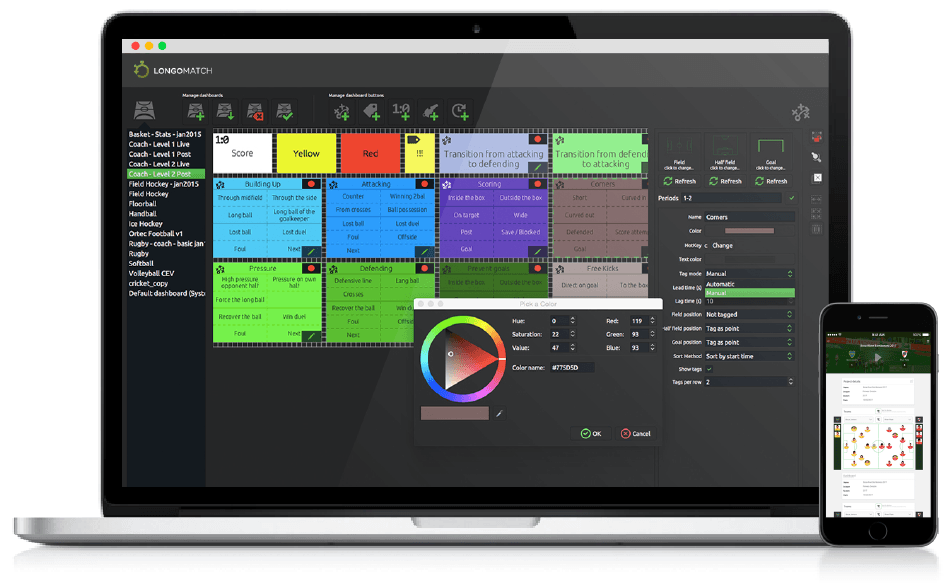
\includegraphics[width=\linewidth]{img/customize_longo.png}
\caption{Customization}
\label{fig:customization_longo}
\end{subfigure}\hfil
\begin{subfigure}{0.33\textwidth}
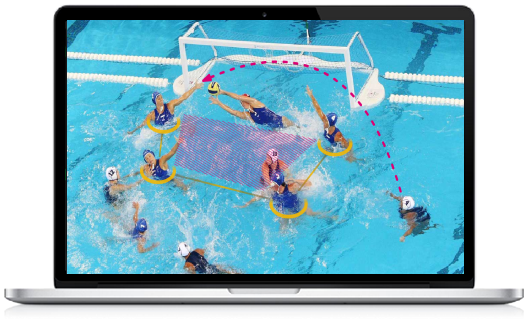
\includegraphics[width=\linewidth]{img/drawing_longo.png}
\caption{Drawing}
\label{fig:drawing_longo}
\end{subfigure}\hfil 
\begin{subfigure}{0.33\textwidth}
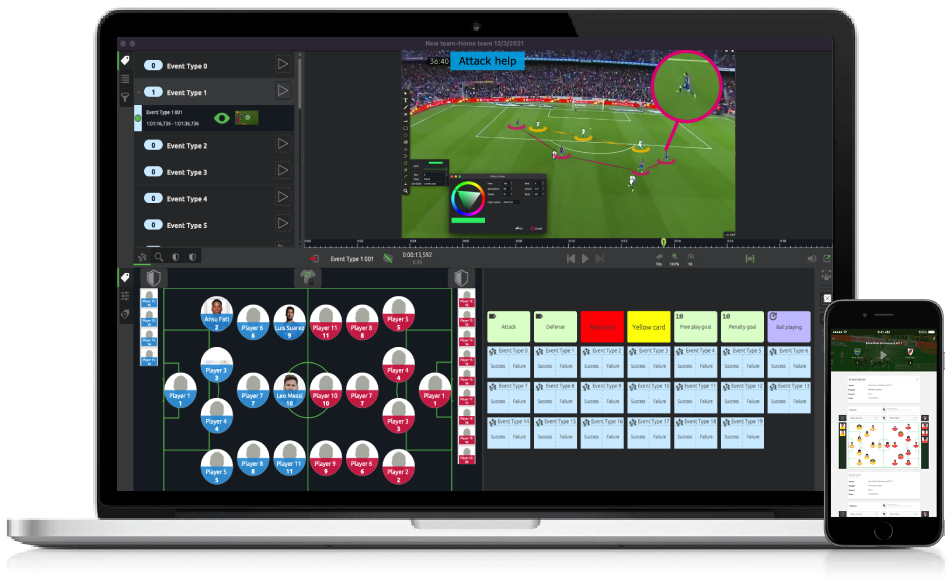
\includegraphics[width=\linewidth]{img/tagging_longo.png}
\caption{Tagging}
\label{fig:tagging_longo}
\end{subfigure}\hfil 
\caption{
\label{fig:analysis_competitor}LongoMatch Functionalities}
\end{figure}

\subsubsection{NAC Sport}
\textit{NAC Sport} \cite{NacSport} è un app con caratteristiche molto simili a quelle di \textit{LongoMatch}. Ciò che la distingue, è la possibiltà di effettuare analisi in \textit{realtime}, fornendo all'utente feedback istantanei. Inoltre supporta il riconoscimento tridimensionale di palla e giocatori, per avere un panorama a 360 gradi di un determinato evento. Come \textit{LongoMatch}, implementa funzionalità di tagging eventi tramite dashboard o shortcut da tastiera preimpostati. Implementa inoltre grafiche interattive, come ad esempio \textit{heatmaps}, per fornire ulteriori dettagli all'utente. Economicamente, \textit{NAC Sport} risulta essere più costoso rispetto ad altre alternative, proprio perchè è stato progettato per soddisfare le esigenze di un target professionale. Questi aspetti rendono \textit{NAC Sport} uno software completo, ma non adatto ad un bacino di utenti amatoriali.

\pagebreak

\subsection{Hybrid Systems}
Gli \textit{Hybrid Systems}, come dice la sigla stessa, combinano software di analisi video e tecnologie esterne. Alcuni esempi di hardware integrativi sono i dispositivi wearable, i sensori e le telecamere specializzate. Questi sistemi risultano estremamente efficienti perchè suddivisi in due fasi. Inizialmente, l'utilizzo di sensori permette di monitorare molti parametri che, successivamente, vengono utilizzati ed integrati nella fase di analisi video per avere risultati più precisi. 
\noindent Di seguito sono presentate ed illustrate 2 soluzioni leader nel settore.

\subsubsection{Hudl}
\label{subsubsec:hudl}
\begin{wrapfigure}{r}{0.48\textwidth}
    \centering
    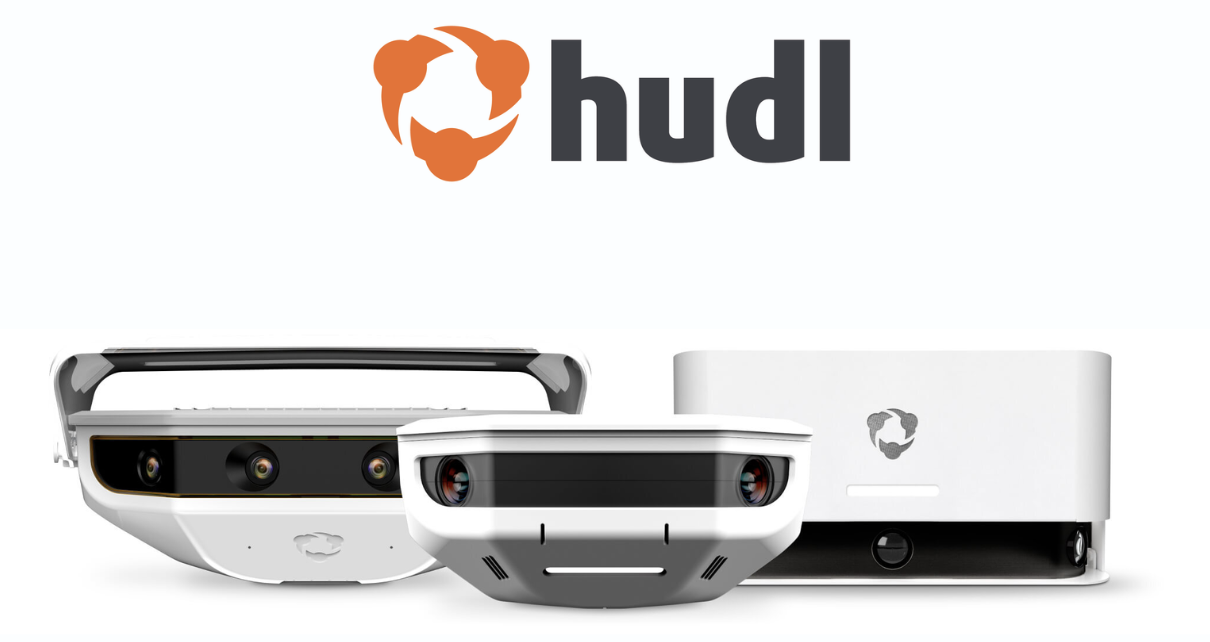
\includegraphics[scale=0.4]{img/hudl_focus.png}
    \caption{Hudl Focus}
    \label{fig:Hudl Focus}
\end{wrapfigure}
Hudl \cite{Hudl} è una piattaforma di analisi video sportiva, utilizzata da oltre \textit{8 milioni} di utenti registrati e \textit{230.000 squadre} in più di \textit{40 sport}, con \textit{16 milioni} di download dell'app.

\noindent Hudl offre una vasta gamma di prodotti innovativi per rispondere alle esigenze del mondo dello \textit{Sport 4.0}. I principali sono: \textit{Sportscode}, \textit{Volleymetrics}, \textit{Assist}, \textit{WIMU} e \textit{Hudl Focus}.

\noindent Proprio quest'ultimo è il servizio di punta dell'azienda, che integra l'analisi video con l'utilizzo di telecamere progettate da Hudl stessa.  In particolare l'azienda ha sviluppato software dedicati che permettono alle camere di seguire le azioni live in maniera automatica, offrendo una soluzione completamente \textit{hands-free}. Hudl Focus utilizza queste camere intelligenti per registrare ogni momento del gioco senza interventi manuali. Questo servizio è particolarmente utilizzato negli sport in cui il campo di gioco è ampio, ad esempio calcio o football americano.




\subsubsection{Catapult}
\label{subsubsec:catapult}
\begin{wrapfigure}{r}{0.48\textwidth}
    \centering
    \vspace{-15px}
    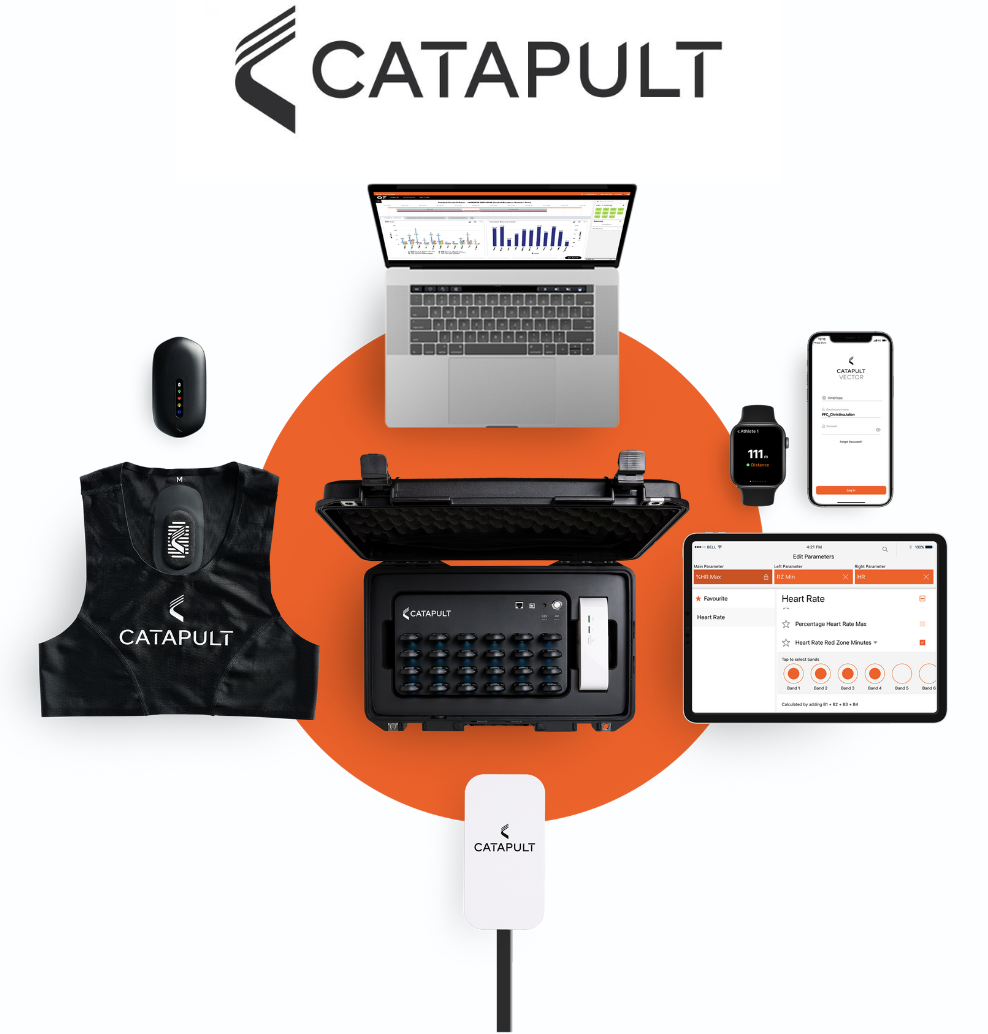
\includegraphics[scale=0.48]{img/catapult.png}
    \caption{Catapult Vector Core}
    \label{fig:Catapult Vector Core}
\end{wrapfigure}
Catapult \cite{Catapult} è una piattaforma leader nel monitoraggio e nell'analisi sportiva, utilizzati da oltre \textit{4.200 squadre} in più di \textit{40 sport} in tutto il mondo. Uno dei loro prodotti di punta è \textit{Vector Core}.

Questa soluzione fornisce pettorine con tecnologie GPS/GNSS  per tracciare i movimenti degli atleti, fornendo dati in \textit{realtime} ma anche post-sessione. Il prodotto ha riscosso grande successo perchè facile da configurare e offre un'ampia gamma di metriche per l'analisi delle prestazioni fisiche. 

\noindent Le caratteristiche principali di Vector Core includono:
\begin{itemize}
    \item \textit{Tracciamento integrato indoor e outdoor}
    \item \textit{Tecnologia GPS/GNSS a 10 Hz}
    \item \textit{Analisi inerziale del movimento}
    \item \textit{Compatibilità con monitoraggio della frequenza cardiaca}
    \item \textit{Reportistica dettagliata con oltre 200 parametri live e 1.800 parametri post-sessione}
\end{itemize}

\subsection{Volleyball Specific}
Alcune aziende si sono specializzate nel fornire soluzioni verticali per specifici sport, come la pallavolo. Di seguito analizziamo due esempi rilevanti.

\subsubsection{DataVolley 4.0}
DataVolley 4.0 \cite{Data-Volley4.0} è uno dei prodotti di riferimento nella pallavolo internazionale ed è sviluppato dall'azienda Data Project. Il software è progettato per la raccolta e analisi di dati di partite ed allenamenti. Il suo punto di forza risiede nell'interfaccia per la raccolta dei dati (molto simile alla stenografia) e nelle successive funzioni che permettono di generare report e statistiche relative alle squadre e ad ogni singolo giocatore associando anche il video. L'applicazione è focalizzata in particolare alla raccolta dei dati delle performance e non all'analisi dei singoli fondamentali (e quindi la tattica). Inoltre richiede un po' di addestramento per imparare ad utilizzarlo, per cui utenti amatoriali finiscono per non farne uso anche se esistono versioni economiche.


\subsubsection{BallTime}
BallTime \cite{BallTime} è una startup NewYorkese che sfrutta modelli di Computer Vision per l'analisi video. In particolare i modelli di ML riescono a:
\begin{itemize}
    \item Riconoscere e distinguere i singoli giocatori
    \item Tracciare la palla
    \item Analizzare pattern di gioco
    \item Riconoscere azioni e segnare il risultato
\end{itemize} 

La startup, nata a Settembre 2022, fornisce una web app completa, ma ancora in costante sviluppo. Infatti questa soluzione sta introducendo le funzionalità di volta in volta guidata dalla domanda. L'approccio innovativo e soprattutto \textit{user-friendly}, il prezzo contenuto e l'attività di marketing che l'azienda sta sviluppando, rendono \textit{BallTime} una soluzione competitiva dove le alternative dovranno puntare su funzioni diverse o strategie di creazione di comunità.


      \newpage
      \chapter{Analisi e progettazione}
\label{cha:analisi_progettazione}

Analizzando i vari competitor descritti nel precedente capitolo, si può notare che la maggior parte delle soluzioni presenti sul mercato sono rivolte ad una clientela qualificata. Questo probabilmente per avvicinarsi ad un utenza con più disponibilità economica.
Anche soluzioni come \textit{LongoMatch}, che offrono funzionalità più semplici, non sono progettate per un utilizzo amatoriale.

In seguito a queste analisi, ho deciso di sviluppare un'applicazione orientata ad un unico sport che fosse estremamente \textit{user-friendly}, con un'interfaccia intuitiva e con un set di funzionalità relativamente limitato. Ho deciso di focalizzarmi sulla pallavolo, uno sport che ho praticato per quasi 10 anni. Le caratteristiche di questo sport lo rendono ideale per l'analisi video, in quanto vi sono pochi giocatori e il campo ha dimensioni ridotte. Questo permette di avere una visione chiara di tutte le dinamiche di gioco, rendendole facilmente analizzabili.

La soluzione proposta è caratterizzata da un'interfaccia utente estremamente intuitiva, ideata per essere facilmente utilizzabile da utenti amatoriali. Inoltre, seguendo l'esempio della start-up \textit{BallTime}, oltre alle comuni funzionalità di analisi, ho implementato alcune funzionalità AI offrendo quindi due modalità di uso: Manuale e AI.

Le due modalità si distinguono in questo modo:
\begin{itemize}
    \item \textbf{Manuale}: Questa modalità permette di creare, importare ed esportare progetti. In particolare sono implementate le funzionalità di:
    \begin{itemize}
        \item \textit{Event Tagging}: che offre la possibilità di salvare eventi d'interesse durante l'analisi video. Sono caratterizzati dall'utilizzo di shortcut personalizzabili secondo atleta, azione e comando rapido.
        \item \textit{Drawing Tools}: attraverso cui è possibile annotare ed illustrare tattiche o azioni di gioco direttamente sul frame video.
        \item \textit{Videoclip Generator}: per generare highlights in maniera completamente automatica, partendo dagli eventi taggati. 
    \end{itemize}
    \item \textbf{AI}: Questa modalità implementa l'utilizzo di modelli di Computer Vision per l'analisi automatica dei video. In particolare sono implementate le funzionalità di:
    \begin{itemize}
        \item \textit{Ball Trajectory}: visualizzazione della traiettoria della palla durante il gioco. Disegnando una scia gialla sul video.
        \item \textit{Player Recognition}: per identificare automaticamente i giocatori in campo, assegnando ad ognuno un id e un colore di bounding box diverso.
    \end{itemize}   
\end{itemize}

\noindent I risultati dell'analisi di mercato hanno inoltre evidenziato che i prodotti si suddividono in due categorie: \textit{Desktop App} e \textit{Web App}.
Al fine di favorire il riuso su più scenari ho deciso di creare una Web App che, oltre a poter essere disponibile su un server, può essere eseguita su un computer in locale permettendo quindi scenari di servizio in cloud o di riuso su una propria macchina dedicata senza necessità di creazione di utenze

\section{Perché una Web App?}
\label{sec:web_app}

La decisione di sviluppare una Web App invece che una desktop app è basata su diversi fattori.

Una prima analisi ha delineato come l'utilizzo di siti web risulti più semplice per un target di utenza amatoriale. Questo perchè non richiede l'installazione secondo sistemi operativi specifici e può essere eseguita su un qualsiasi browser.

Questo rende l'accesso all'app semplice ed immediato, creando un'esperienza più \textit{user-friendly} con meno problematiche sul fronte della configurazione. Inoltre, offrendo potenzialmente il servizio in cloud, diventa molto più facile la gestione degli aggiornamenti in quanto saranno sempre centralizzati, rendendo l'esperienza utente più semplice e lontana da noiose installazioni manuali necessarie a garantire sempre l'ultima versione.


Un ulteriore vantaggio viene dalla funzionalità AI. Infatti, l'uso di modelli di Computer Vision richiedono risorse computazionali che non sempre sono disponibili a chiunque, sviluppando l'applicazione con interfaccia web  è possibile fare uso di tecniche di \textit{cloud computing} in cui è possibile delegare i processi computazionalmente intensi a server remoti. Questo garantisce una \textit{user-experience} il più fluida e performante possibile.

Pertanto, seguendo la volontà di creare un prodotto semplice e con basse problematiche agli utenti finali, l'approccio web è risultato quello vincente, dato che il bacino di utenza a cui si rivolge è quello di utenti amatoriali con poche disponibilità di tempo e di risorse. 

\section{Analisi dei Requisiti}
\label{sec:requisiti}

La Web App ha lo scopo di rivolgersi ad un target non professionale, quali atleti ed allenatori amatoriali. Identificandosi in questa utenza, sono state studiate le soluzioni già presenti e le funzionalità da loro proposte. In particolare, sono state prese in considerazione le feature di \textit{LongoMatch} e \textit{BallTime}, successivamente rivisitate e adattate per una \textit{user-experience} orientata a rendere il tutto più facile. 

\noindent In fase di analisi è stato fondamentale definire quelli che sono i requisiti funzionali e non funzionali del sistema.
\subsection{Requisiti Funzionali}
\label{subsec:requisiti_funzionali}

La definizione dei Requisiti Funzionali è fondamentale in fase di analisi. Ci permette infatti di identificare le funzionalità chiave che il sistema deve garantire all'utente finale. Inoltre è utile per fare un brainstorming sulla direzione che il progetto dovrà prendere.

\noindent Di seguito sono elencati i requisiti funzionali del sistema, suddivisi per categorie:

\begin{itemize}
    \item \textbf{Gestione Progetti}
    \begin{itemize}
        \item Gli utenti devono poter creare nuovi progetti, scegliendo video, giocatori e azioni.
        \item Gli utenti devono poter esportare progetti.
        \item Gli utenti devono poter importare progetti esistenti.
    \end{itemize}

    \item \textbf{Modalità e Navigazione}
    \begin{itemize}
        \item Gli utenti devono poter scegliere tra due pagine. Una gestisce l'analisi manuale e l'altra le funzionalità AI.
        \item Gli utenti devono poter navigare tra le due modalità in qualsiasi momento.
    \end{itemize}

    \item \textbf{Analisi Manuale}
    \begin{itemize}
        \item Gli utenti devono poter etichettare eventi di loro interesse durante l'analisi video.
        \item Gli eventi etichettati devono essere personalizzabili e la loro attivazione deve essere rapida.
        \item Gli eventi etichettati devono salvare dati su giocatore, azione, minutaggio e comando rapido associato.
        \item Gli eventi etichettati devono essere valutabili.
        \item Gli utenti devono poter disegnare sui frame video.
        \item Gli utenti devono poter scegliere di creare videoclip partendo degli eventi etichettati.
    \end{itemize}

    \item \textbf{Analisi AI}
    \begin{itemize}
        \item Gli utenti devono poter scegliere tra due modalità di analisi.
        \item Gli utenti devono poter visualizzare i risultati di queste analisi.
        \item Gli utenti devono poter scaricare i risultati delle analisi AI.
    \end{itemize}
\end{itemize}

\subsection{Requisiti Non Funzionali}

Lo scopo dei Requisiti Non Funzionali è quello di descrivere le caratteristiche del software che non sono definite in termini di funzionalità. Questi requisiti riguardano il funzionamento del sistema e i vincoli da rispettare per un prodotto di qualità.

\noindent Di seguito sono elencati i principali requisiti non funzionali del sistema, suddivisi in tre macroaree:

\begin{itemize}
    \item \textbf{Prestazioni}
    \begin{itemize}
        \item L'app deve garantire l'elaborazione video in tempi brevi.
        \item L'app deve essere estremamente reattiva agli input dell'utente.
    \end{itemize}

    \item \textbf{Usabilità}
    \begin{itemize}
        \item L'app deve garantire una \textit{UX} fluida e dinamica.
        \item L'app deve avere una \textit{UI} chiara ed intuitiva. 
    \end{itemize}

    \item \textbf{Compatibilità}
    \begin{itemize}
        \item L'app deve essere compatibile con i principali browser web.
        \item L'app deve adattarsi a diverse dimensioni di schermo.
    \end{itemize}
\end{itemize}

\section{Progettazione}
\label{sec:progettazione}

La progettazione della Web App ha mantenuto il focus sull'esperienza utente. Proprio per questo motivo ho creato un \textit{mockup} dell'interfaccia dell'app utilizzando Figma. 
Per avere una visione più approfondita di comportamenti e abitudini del target, ho definito due \textit{personas} e due \textit{scenari}. Durante lo sviluppo dell'applicazione ho progettato \textit{UX} e \textit{UI}, tenendo conto di questi preconcetti. 






\subsection{Personas e Scenari}
\label{subsec:personas_scenari}
\noindent Le \textit{personas} sono personaggi inventati che rappresentano possibili utenti reali. Gli \textit{scenari}, invece, descrivono dettagliatamente delle situazioni specifiche in cui l'app potrebbe essere utilizzata.
In fase di progettazione e sviluppo del prototipo Figma, definire questi concetti mi ha aiutato a capire come il target potrebbe interagire con l'applicazione.

\subsubsection{Personas}

\begin{itemize}
    \item \textbf{Marco}, 45 anni, vive a Trento ed è allenatore di una delle squadra di pallavolo Under-16 della provincia. Durante le partite è solito annotare con carta e penna le sue considerazioni rispetto alle prestazioni della squadra. Proprio a causa di questo però, gli capita spesso di perdere fasi di gioco importanti. Gli piacerebbe, quindi, poter registrare le partite, per poi fare le sue valutazioni a casa.  
     
    \item \textbf{Gaia}, 22 anni, vive a Modena ed è una giocatrice di pallavolo in una squadra universitaria. Durante le partite è solita registrarsi, chiedendo poi a suo fratello, una volta a casa, di creare highlights delle sue migliori azioni. A Gaia da fastidio non poter essere autonoma, ma proprio non riesce a prendere praticità con le app di editing video e non trova nessuna altra soluzione.
\end{itemize}

\subsubsection{Scenari}


\begin{itemize}
    \item \textbf{Scenario A}: Durante un time-out, l'allenatore raduna i giocatori attorno alla panchina. Mostra sul suo tablet il video dell'azione appena conclusa utilizzando VolleyVisionAI e con un pennino inizia a disegnare sul video, evidenziando movimenti e possibili tattiche. I giocatori hanno così istruzioni chiare su come procedere, tornando in campo più consapevoli e preparati.
    \item \textbf{Scenario B}: Prima di una gara importante, l'allenatore decide di convocare la squadra per sviluppare insieme un piano di gioco. Tramite l'utilizzo di VolleyVisionAI l'allenatore si è preparato il giorno prima dei video di alcune fasi di gioco della squadra avversaria. Successivamente ha mostrato i videoclip ai giocatori per poi interrogarli su come avrebbero reagito in determinate situazioni. Questa sessione di confronto ha permesso di migliorare l'intesa di squadra e di prepararsi per la gara.
\end{itemize}

\subsection{Struttura e Interfaccia}
\label{subsec:interfaccia}

L'utilizzo di Figma per la creazione di un prototipo della \textit{User Interface} ha permesso di capire come impostare la struttura della Web App. Il corso di \textit{EyeStudios Academy} mi ha fornito le competenze tecniche necessarie per la creazione del mockup.

VolleyVisionAI è stato ideato per avere un menu principale con due opzioni, come già descritto nell'introduzione di questo capitolo. Entrambe le funzionalità redirigono l'utente ad una nuova pagina, di seguito descritte.

La prima funzionalità, \textit{Manual}, è stata strutturata in modo da rendere chiari i tre componenti principali. Sulla destra troviamo il video player con sotto un box contenente due campi utili alla creazione degli shortcut. Sulla sinistra, invece, troviamo il contenitore di tutti gli eventi taggati fino a quel momento. Questa struttura offre una \textit{User Interface} e \textit{User Experience} semplice ed intuitiva. 

La seconda funzionalità, \textit{AI}, presenta invece un video player quasi a tutto schermo con sopra la descrizione di ciò che viene rappresentato. Questa interfaccia minimalista aiuta l'utente a concentrarsi unicamente sul risultato dell'analisi AI. 

La Web App presenta come colore predominante l'azzurro, scelto poichè trasmette tranquillità e professionalità. Inoltre le sue sfumature rendono ben leggibili i vari componenti dell'interfaccia e, allo stesso tempo, non stancano l'occhio dell'utente. In fase di progettazione, ho notato come l'azzurro fosse ideale per rappresentare il connubio tra sport e tecnologia: evoca dinamismo ed energia, tipici dello sport, e trasmette al contempo freschezza e innovazione, caratteristiche della tecnologia. Così, l'azzurro bilancia intensità e modernità, rendendo l'interfaccia armoniosa ed efficace.

\begin{figure}[htb]
    \centering 
    \begin{subfigure}{0.48\textwidth}
        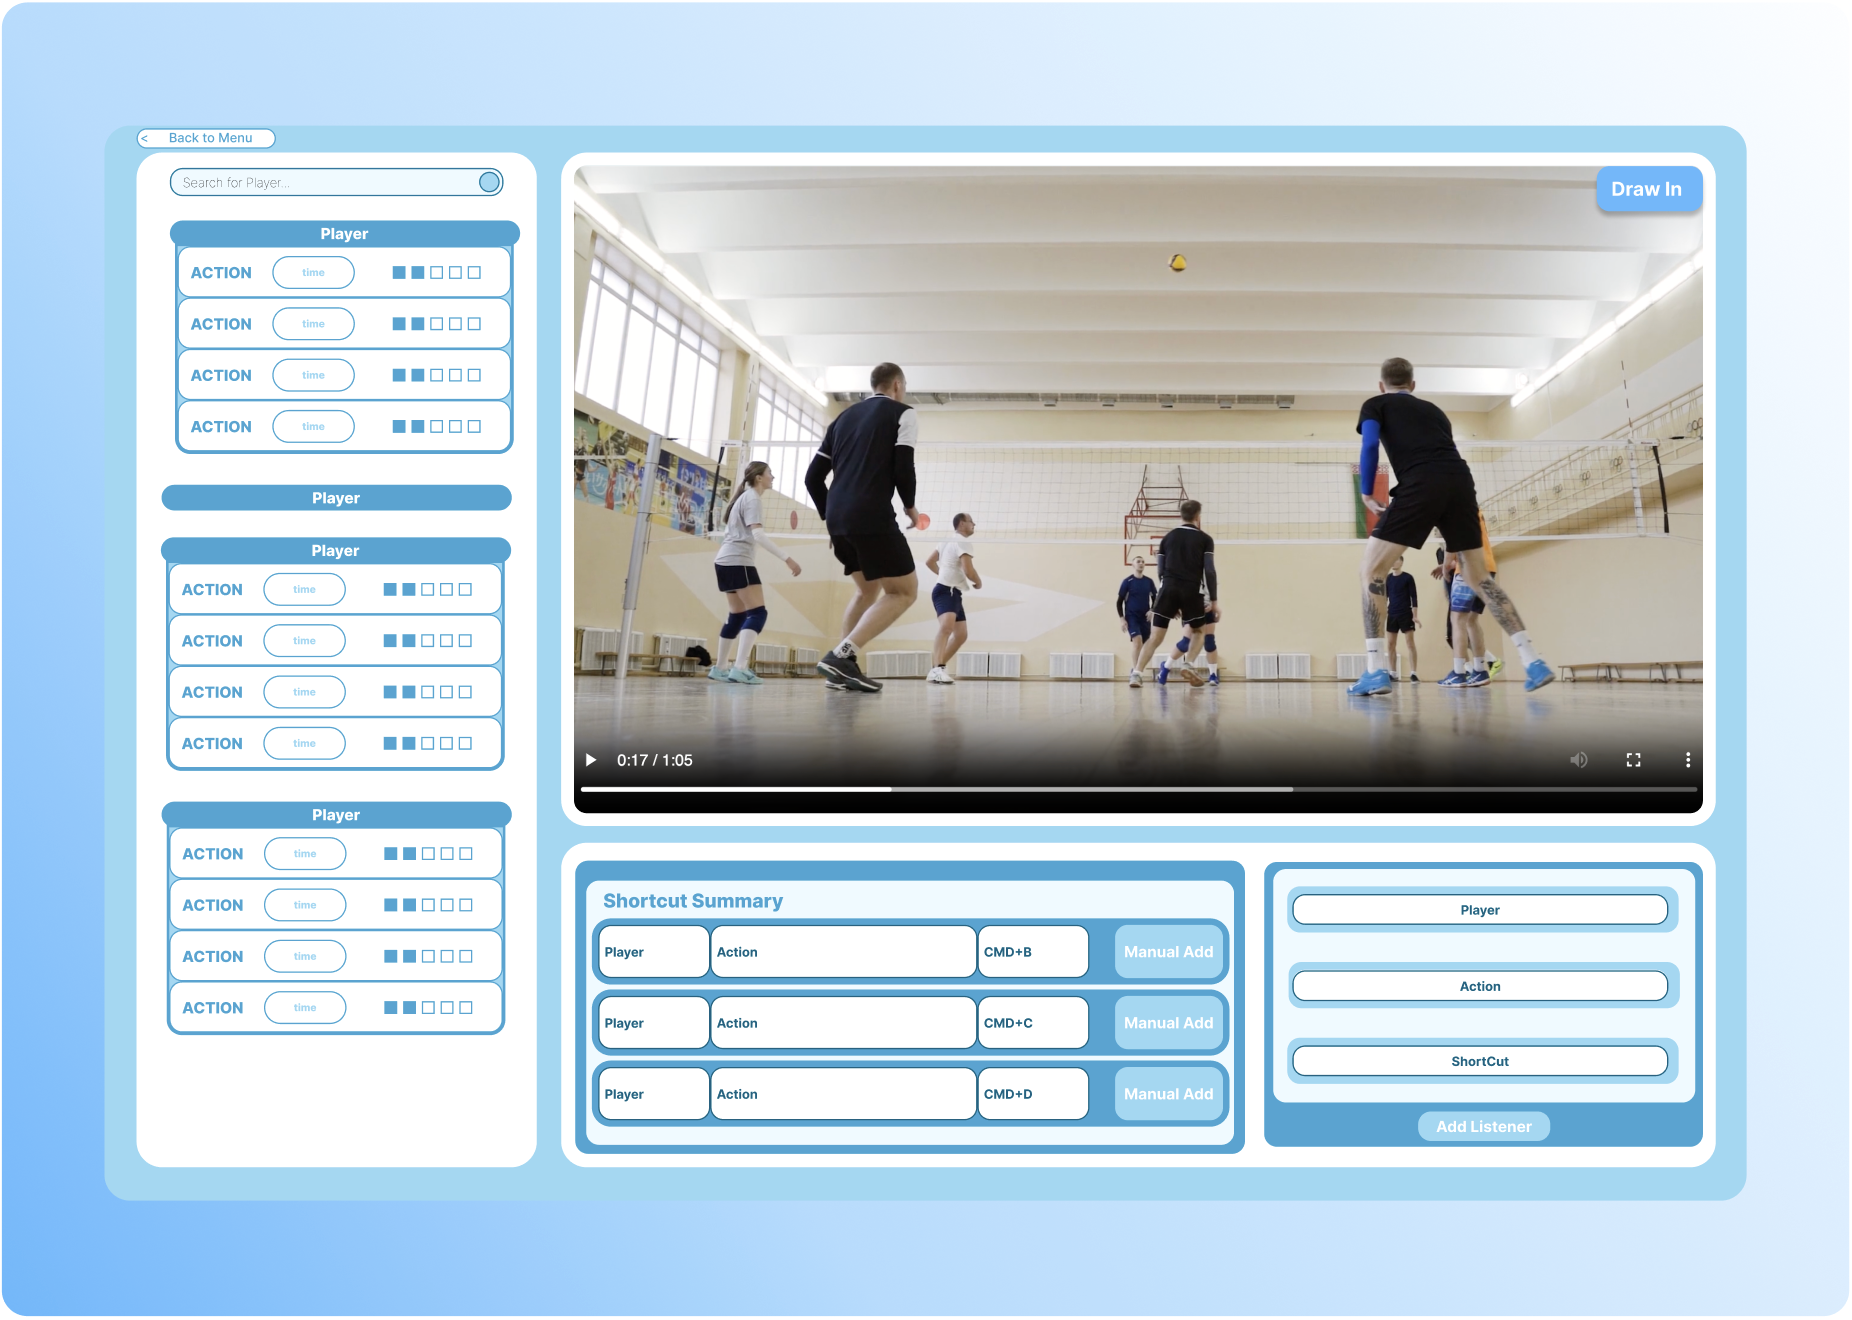
\includegraphics[width=\linewidth]{img/figma_manual.png}
        \caption{Mockup Analisi Manuale}
        \label{fig:mokup_manual}
    \end{subfigure}\hspace{0.04\textwidth}% Aggiunge uno spazio tra le due immagini
    \begin{subfigure}{0.48\textwidth}
        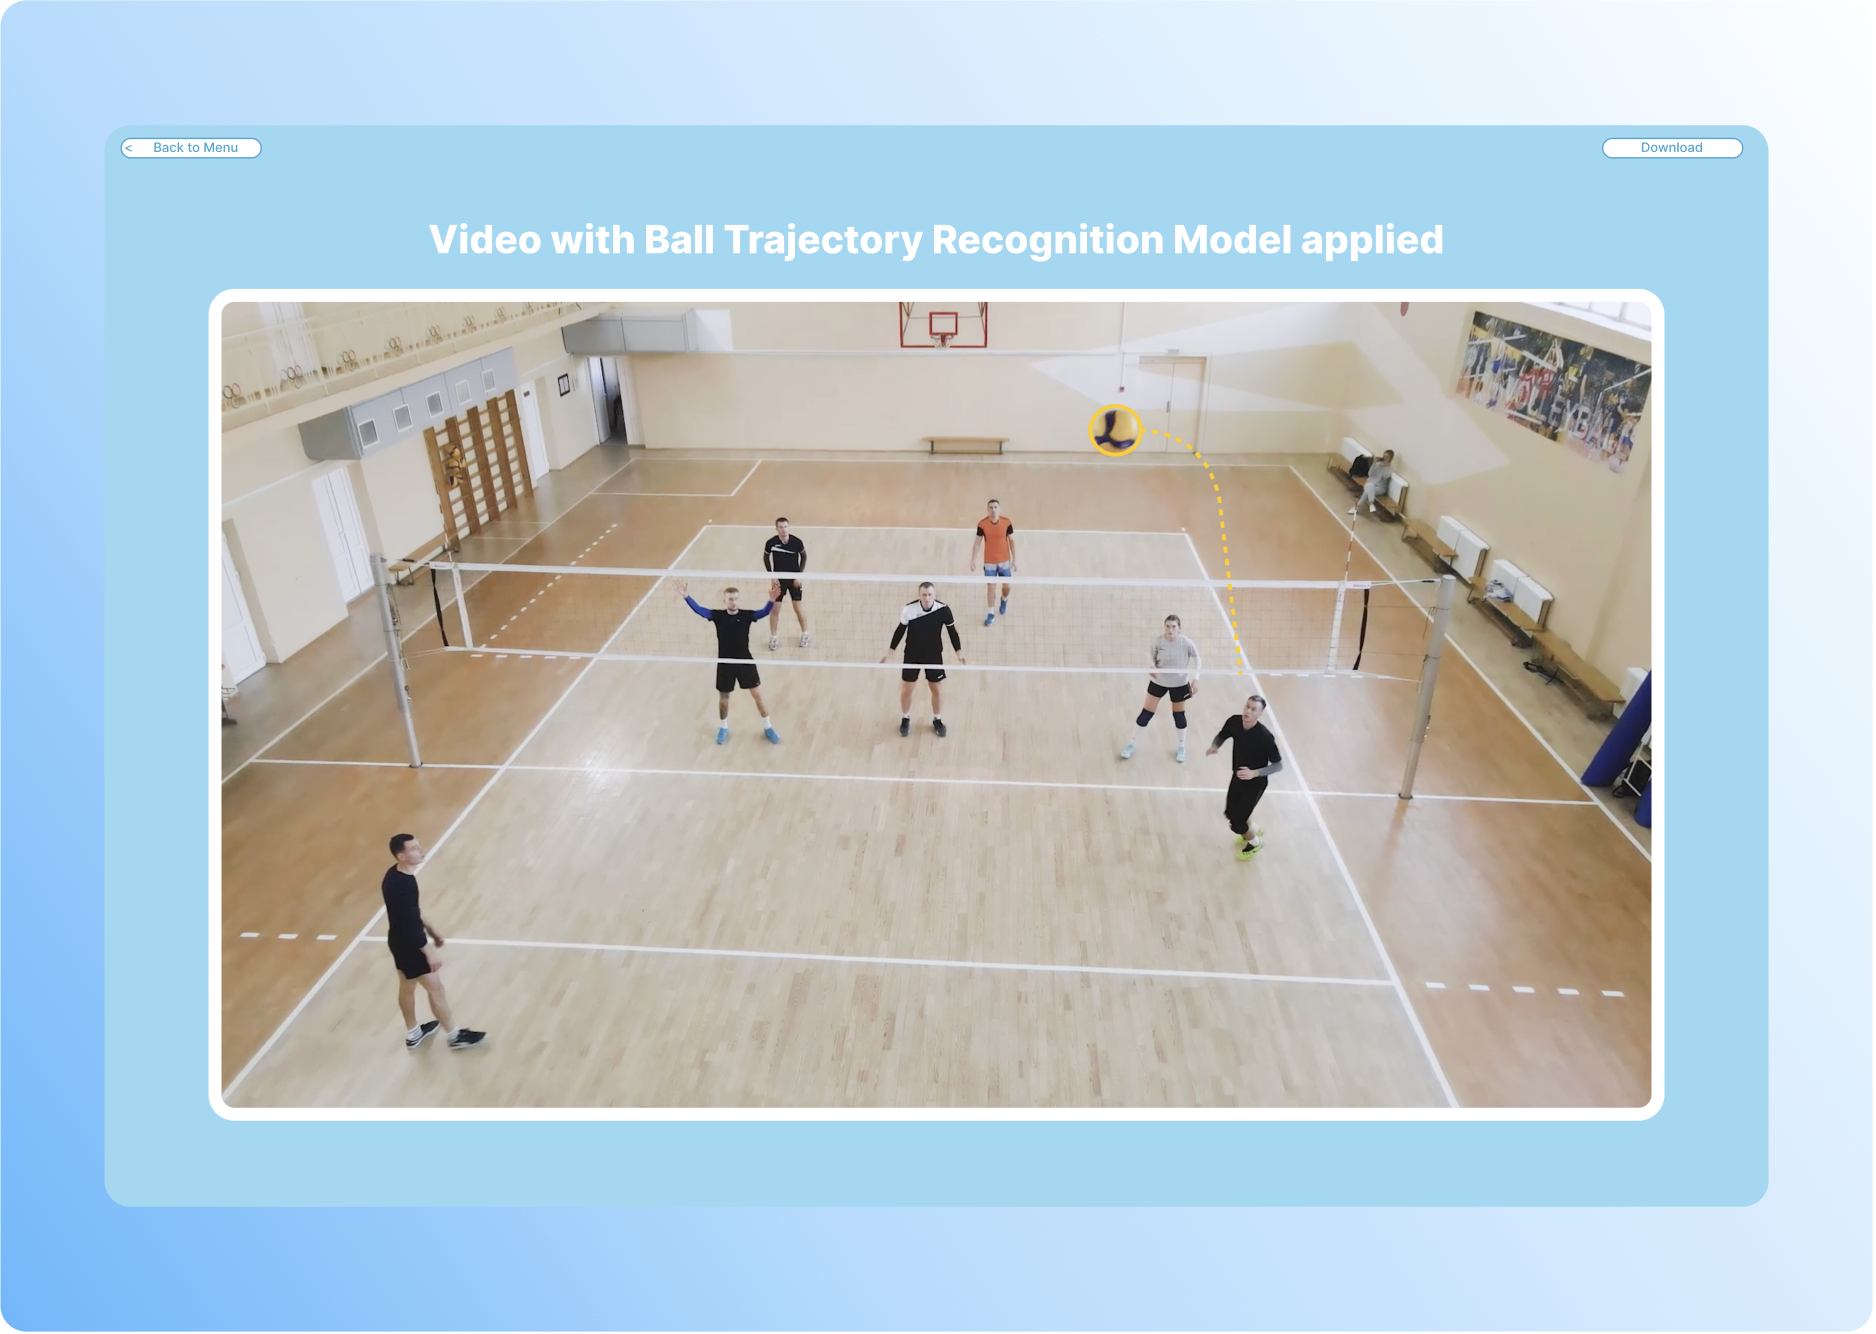
\includegraphics[width=\linewidth]{img/figma_ai.png}
        \caption{Mockup Analisi AI}
        \label{fig:mokup_ai}
    \end{subfigure}
    \caption{Figma Mockup}
    \label{fig:bot_competitor}
\end{figure}

\subsection{Server}
\label{sec:subserver}


Per garantire una manipolazione efficiente dei video e l'implementazione dei modelli di \textit{Computer Vision}, è stato necessario sviluppare un server back-end robusto e affidabile. Questo server svolge un ruolo cruciale nella gestione delle operazioni computazionalmente intensive, liberando i dispositivi degli utenti dal carico di elaborazione e assicurando un'esperienza d'uso fluida e performante.
Il Server è connesso direttamente al front-end della Web App tramite API , consentendo una comunicazione rapida e sicura tra l'interfaccia utente e il back-end. Questo permette di ricevere richieste, elaborare i dati dei video tramite i modelli di \textit{Computer Vision} e restituire i risultati all'utente in tempo reale.

      \newpage
      \chapter{Sviluppo e implementazione}
\label{cha:sviluppo_implementazione}

Il prototipo realizzato con Figma, per quanto semplice, ha permesso di indirizzare da subito i passaggi dello sviluppo: realizzazione del codice del front-end progettato e successiva implementazione dello sviluppo del back-end.

Successivamente viene descritto l'effettivo funzionamento dell'app, con relative illustrazioni, prestando attenzione anche ad architettura e tecnologie utilizzate.

\section{Tecnologie utilizzate}
\label{sec:tecnologie}

Di seguito sono presentate brevemente le varie tecnologie utilizzate per l'implementazione di VolleyVisionAI.


\subsection{Node.js}
\begin{wrapfigure}{r}{0.33\textwidth}
    \centering
    
\includegraphics[scale=0.17]{nodejs.png}
    \caption{Logo NodeJS}
\end{wrapfigure}
    
Node.js è un runtime system in JavaScript orientato agli eventi e completamente Open-Source. Garantisce performance e prestazioni elevate, basandosi sul motore JavaScript V8 di Google Chrome. Node.js è particolarmente valorizzato per il suo accesso a \textit{Node Package Manager}. NPM è un gestore di pacchetti predefinito per l'ambiente di runtime JavaScript Node.js, nonchè il più grande ecosistema di librerie open source al mondo. Questo permette agli sviluppatori di utilizzare soluzioni già pronte condivise dalla community, accelerando le fasi di programmazione e garantendo sicurezza e solidità del codice.


\subsection{React.js}
\begin{wrapfigure}{r}{0.33\textwidth}
    \centering
    \vspace{-15px}
    
\includegraphics[scale=0.15]{react.png}
    \caption{Logo ReactJS}
\end{wrapfigure}
    
ReactJS è una libreria JavaScript, anche essa Open Source, sviluppata da Meta per la costruzione di interfacce utente, particolarmente utilizzato per complesse \textit{User-Interface} e applicazioni a pagina singola. Questa libreria è largamente utilizzata ed apprezzata per il suo vasto ecosistema, che include strumenti come \textit{React Developer Tools} e \textit{Create React App}. Per lo sviluppo della mia app ho adottato proprio quest'ultimo che utilizza \textit{Node.js} e \textit{NPM}, permettendomi di avviare un progetto React in maniera semplice e veloce. Inoltre React è una libreria che utilizza una struttura basata su componenti, che permettono di creare interfacce riutilizzabili e modulabili


\subsection{Figma}
\begin{wrapfigure}{r}{0.33\textwidth}
    \centering
    \vspace{-20px}
    
\includegraphics[scale=0.20]{figma.png}
    \caption{Logo Figma}
\end{wrapfigure}
    
Figma è uno strumento di design e grafica vettoriale utilizzato per la creazione di mockup e prototipi. Figma si distingue per essere un applicativo Web, ma che permette comunque soluzioni desktop e mobile. L'obiettivo di Figma è quello di permettere la creazione di design facendo particolare attenzione a \textit{User Experience} e \textit{User Interface}, permettendo inoltre la collaborazione \textit{realtime} tra utenti. Figma è stato fondamentale in fase di analisi e progettazione, poichè mi ha permesso di avere un prototipo dell'app prima dell'implementazione effettiva.

\pagebreak


\subsection{Uvicorn}
\begin{wrapfigure}{r}{0.33\textwidth}
    \centering
    \vspace{-10px}
    
\includegraphics[scale=0.15]{uvicorn.png}
    \caption{Logo Uvicorn}
\end{wrapfigure}

Uvicorn è un server ASGI (Asynchronous Server Gateway Interface), ideato e progettato per eseguire applicazioni web asincrone in Python, in maniera leggera e veloce. La sua architettura asincrona lo rende ottimale per lavorare con framework moderni come \textit{FastAPI} e \textit{Starlette}, permettendogli di gestire un elevato numero di richieste simultaneamente senza problemi. La tecnologia HTTP/2 e WebSocket sono supportate da Uvicorn, rendendolo ideale per applicazioni realtime. Uno dei motivi principali per cui ho scelto di utilizzare un server meno conosciuto come questo è la sua compatibilità con \textit{FastAPI}. Queste tecnologie combinate tra loro, mi permettono di avere un server Back-End veloce ma soprattutto scalabile. 


\subsection{FastAPI}
\begin{wrapfigure}{r}{0.33\textwidth}
    \centering
    
\includegraphics[scale=0.18]{fastapi.png}
    \caption{Logo FastAPI}
\end{wrapfigure}
    

FastAPI è un framework web progettato per creare API in Python. Il framework si basa su standard quali, OpenAPI e JSON Schema, che gli permettono di generare documentazione interattiva in maniera completamente automatica. Come descritto in precedenza, FastAPI utilizza \textit{Uvicorn} come server ASGI a cui delega la gestione delle richieste. Questo permette di avere un'applicazione estremamente veloce, una caratteristica fondamentale per le applicazioni web moderne. Inoltre, ho optato per questa soluzione in quanto FastAPI ha una documentazione chiara e completa, che mi ha permesso di utilizzare il framework senza problemi. 


\subsection{YOLOv9 }
\begin{wrapfigure}{r}{0.33\textwidth}
\centering
\vspace{-5px}

\includegraphics[scale=0.4]{Yolo.png}
\caption{Logo Ultralytics}
\end{wrapfigure}

YOLOv9 è un modello di \textit{object-detection} sviluppato da Ultralytics. Questa ultima versione della famiglia YOLO (You Only Look Once), è una delle soluzioni più avanzate presenti al momento sul mercato. YOLOv9 viene presentato in 5 varianti principali che si distinguono per la loro complessità. In particolare differiscono per la quantità di parametri di cui il modello dispone, ovvero, le varianti più complesse faranno rilevamenti più precisi a discapito di una maggiore richiesta computazionale. Nel contesto della mia Web App, avere la possibilità di scegliere quale tra le soluzioni fosse la più adatta al progetto mi ha fatto scegliere YOLOv9 come soluzione.

\subsection{OpenCV}
\begin{wrapfigure}{r}{0.33\textwidth}
\centering
\vspace{-10px}

\includegraphics[scale=0.1]{OpenCv.png}
\caption{Logo OpenCV}
\end{wrapfigure}

OpenCV, acronimo di Open Source Computer Vision, è una libreria per la visione artificiale e l'elaborazione delle immagini. E' scritta in C++ ma ha anche altre interfacce, una di queste è in Python, che ho utilizzato nel mio progetto. Gli strumenti messi a disposizioni da OpenCV vengono integrati con modelli, nel mio caso YOLOv9, utilizzando i loro risultati per elaborare specifiche grafiche video. La libreria è stata scelta per la sua documentazione e versatilità, ideale per uno sviluppatore che come me è alle prime armi con il mondo AI.  
% YOLOv9 è un modello di \textit{object-detection} sviluppato da Ultralytics. Questa ultima versione della famiglia YOLO (You Only Look Once), è una delle soluzioni più avanzate presenti al momento sul mercato. YOLOv9 viene presentanto in 5 varianti principali che si distinguono per la loro complessità. In particolare differiscono per la quantità di parametri di cui il modello dispone, ovviamente una variante più complessa farà rilevamenti più precisi a discapito di una maggiore richiesta di risorse. Nel contesto della mia Web App, avere la possibilità di scegliere quale tra le soluzioni fosse la più adatta al progetto mi ha fatto scegliere Yolov9 come soluzione.

\pagebreak

\section{Implementazione}
\label{sec:implementazione}

L'implementazione rispetta le premesse definite nelle fasi di analisi e progettazione, concentrandosi sul mantenere una \textit{User Interface} pulita e un'architettura solida e scalabile.
Attualmente la Web App non è ospitata pubblicamente (Deploy) in quanto ancora in fase di sviluppo.
Lo sviluppo principale è stato lato Front-End implementando tutte le funzionalità definite nel capitolo \ref{cha:analisi_progettazione}. Per l'avvio ho utilizzato \textit{create-react-app} necessario a creare l'ambiente di sviluppo. Questo configura in maniera autonoma, tramite l'utilizzo di  \textit{webpack-dev-server}, un server di sviluppo basato su \textit{Node.js} che serve un interfaccia \textit{React} sul browser locale offrendo così un ambiente caratterizzato dal \textit{live reloading}, utile per vedere i cambiamenti apportati nel codice in \textit{real time}. 
La componente \textit{UnifiedContext.js} è stata utilizzata per centralizzare la gestione dello stato della Web App. In questo modo vengono salvati i dati inseriti dall'utente durante l'utilizzo dell'applicazione, come atleti, azioni, shortcut attivati ed eventi taggati. 
Nel Front-End sono implementate tutte le funzionalità ad eccezione di quelle che richiedono maggiori risorse computazionali (es la manipolazione di video o l'applicazione di modelli AI) in quanto delegate tramite API ad un server \textit{Back-End} esterno.
Questo approccio \textit{Multi Server} è stato pensato per alleggerire il lavoro lato client e garantire una maggiore scalabilità in ottica degli sviluppi futuri dell'applicazione.
Questa componente server Back-End è stata sviluppata in Python tramite il pacchetto Python \textit{FastAPI} supportato a sua volta dal server ASGI \textit{Uvicorn}. La scelta di questo Framework (vedi \ref{sec:tecnologie}) ha permesso di creare API in maniera semplice.
L'implementazione con FastAPI gestisce due funzionalità principali: la creazione di videoclip e l'applicazione di modelli AI. Nella prima viene utilizzato il modulo \textit{moviepy} che permette l'\textit{editing} di video. Mentre, per la seconda si è scelto il modello YOLOv9 nella variante YOLOv9c in quanto adatta alla complessità di object-detection che necessita la Web App. L'uso del modello è delegato alla libreria OpenCV con la sua implementazione Python, che permette la gestione grafica dei risultati. Per l'identificazione dei singoli atleti in campo è stato utilizzato l'algoritmo \textit{SORT} (Simple Online and Realtime Tracking), che ha permesso di mantenere l'identità dei singoli per tutta la durata del video.  

\subsection{Architettura}
\label{sec:architettura}

L'architettura di sviluppo della Web App è rappresentata in figura \ref{fig:architettura_app}.

\begin{figure}[h]
    \centering
    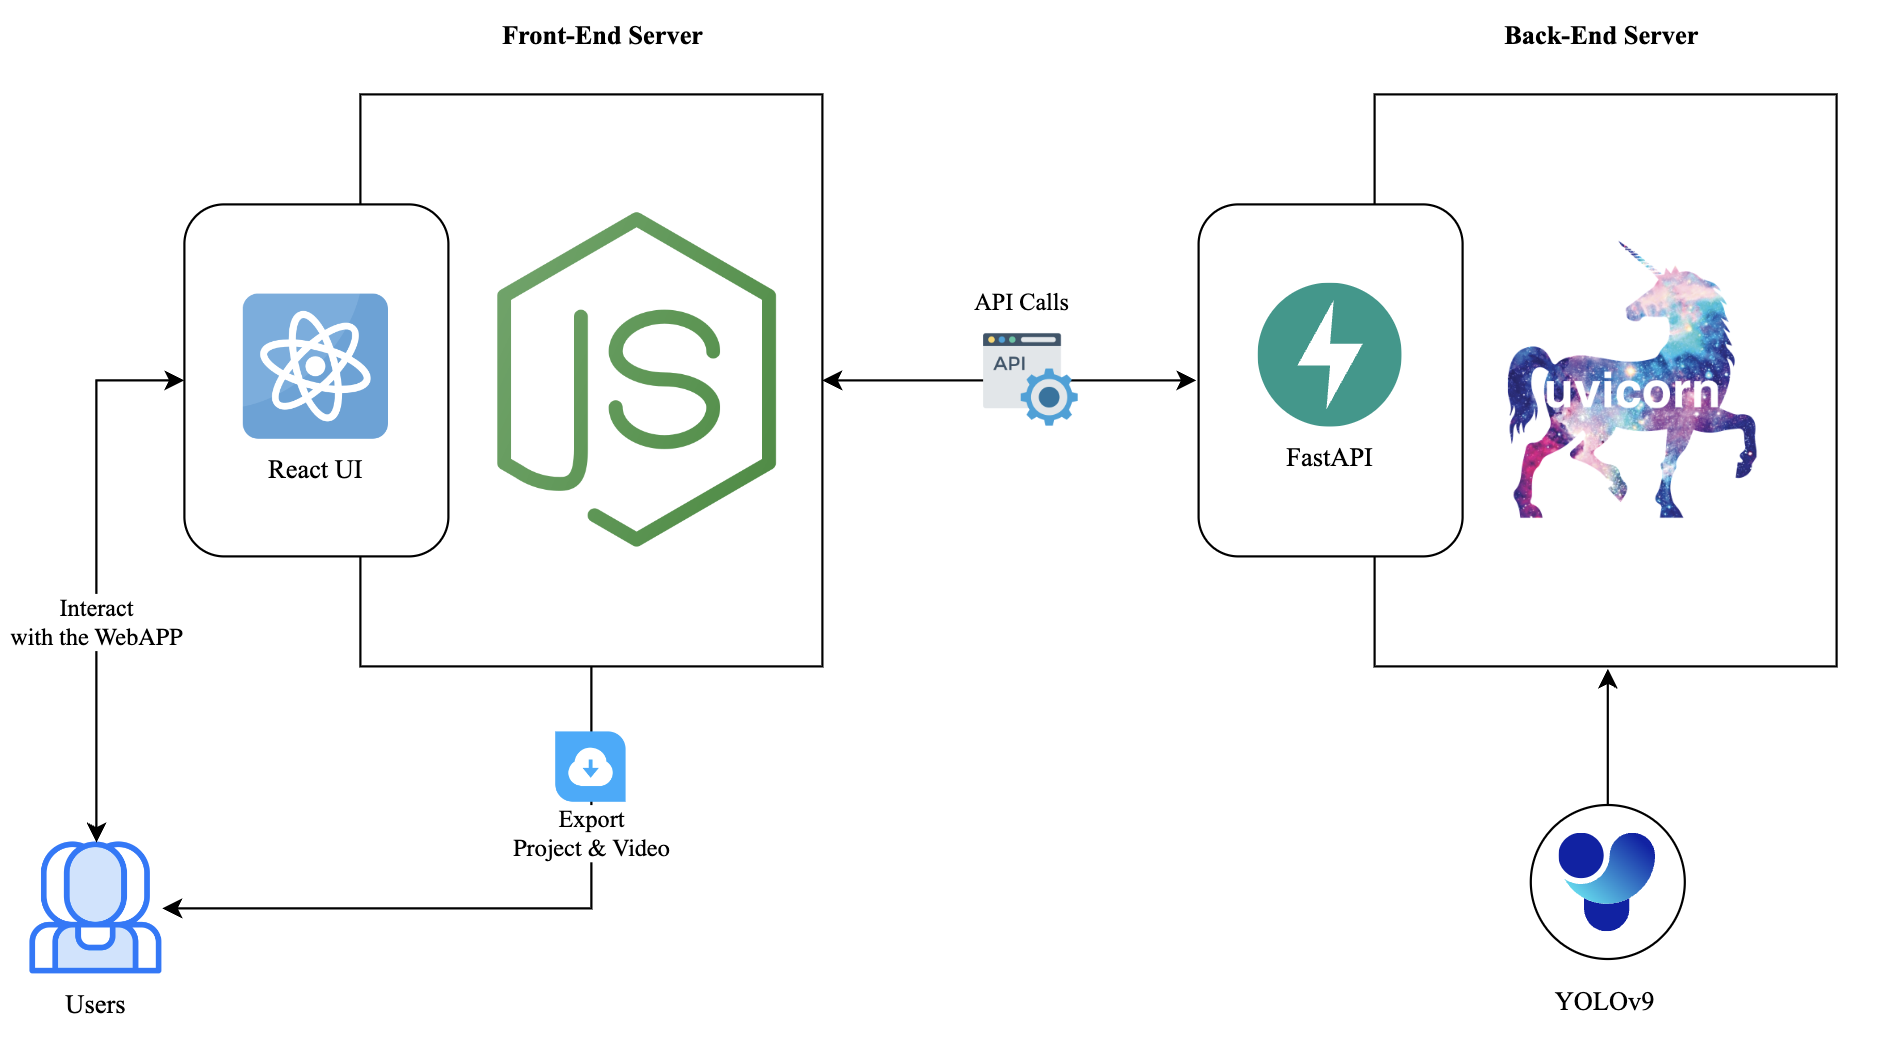
\includegraphics[width=1.02\textwidth]{Architettura.png}
    \caption{Architettura Web App}
    \label{fig:architettura_app}
\end{figure}







\section{UI e Funzionamento Web App}
\label{sec:funzionamento}

Nel seguente paragrafo vengono presentate le funzionalità dell'app mantenendo un ordine logico di navigazione.


\subsection{Menu iniziale}
\label{sec:menu_iniziale}

Il menu iniziale è la prima schermata a cui si accede lanciata la Web App. Questo ha la funzione di guidare l'utente attraverso le modalità base dell'applicazione. Il menu presenta il logo della Web App con le due principali opzioni d'uso: \textit{Manual} ed \textit{AI}.


\begin{figure}[h]
    \centering
    \frame{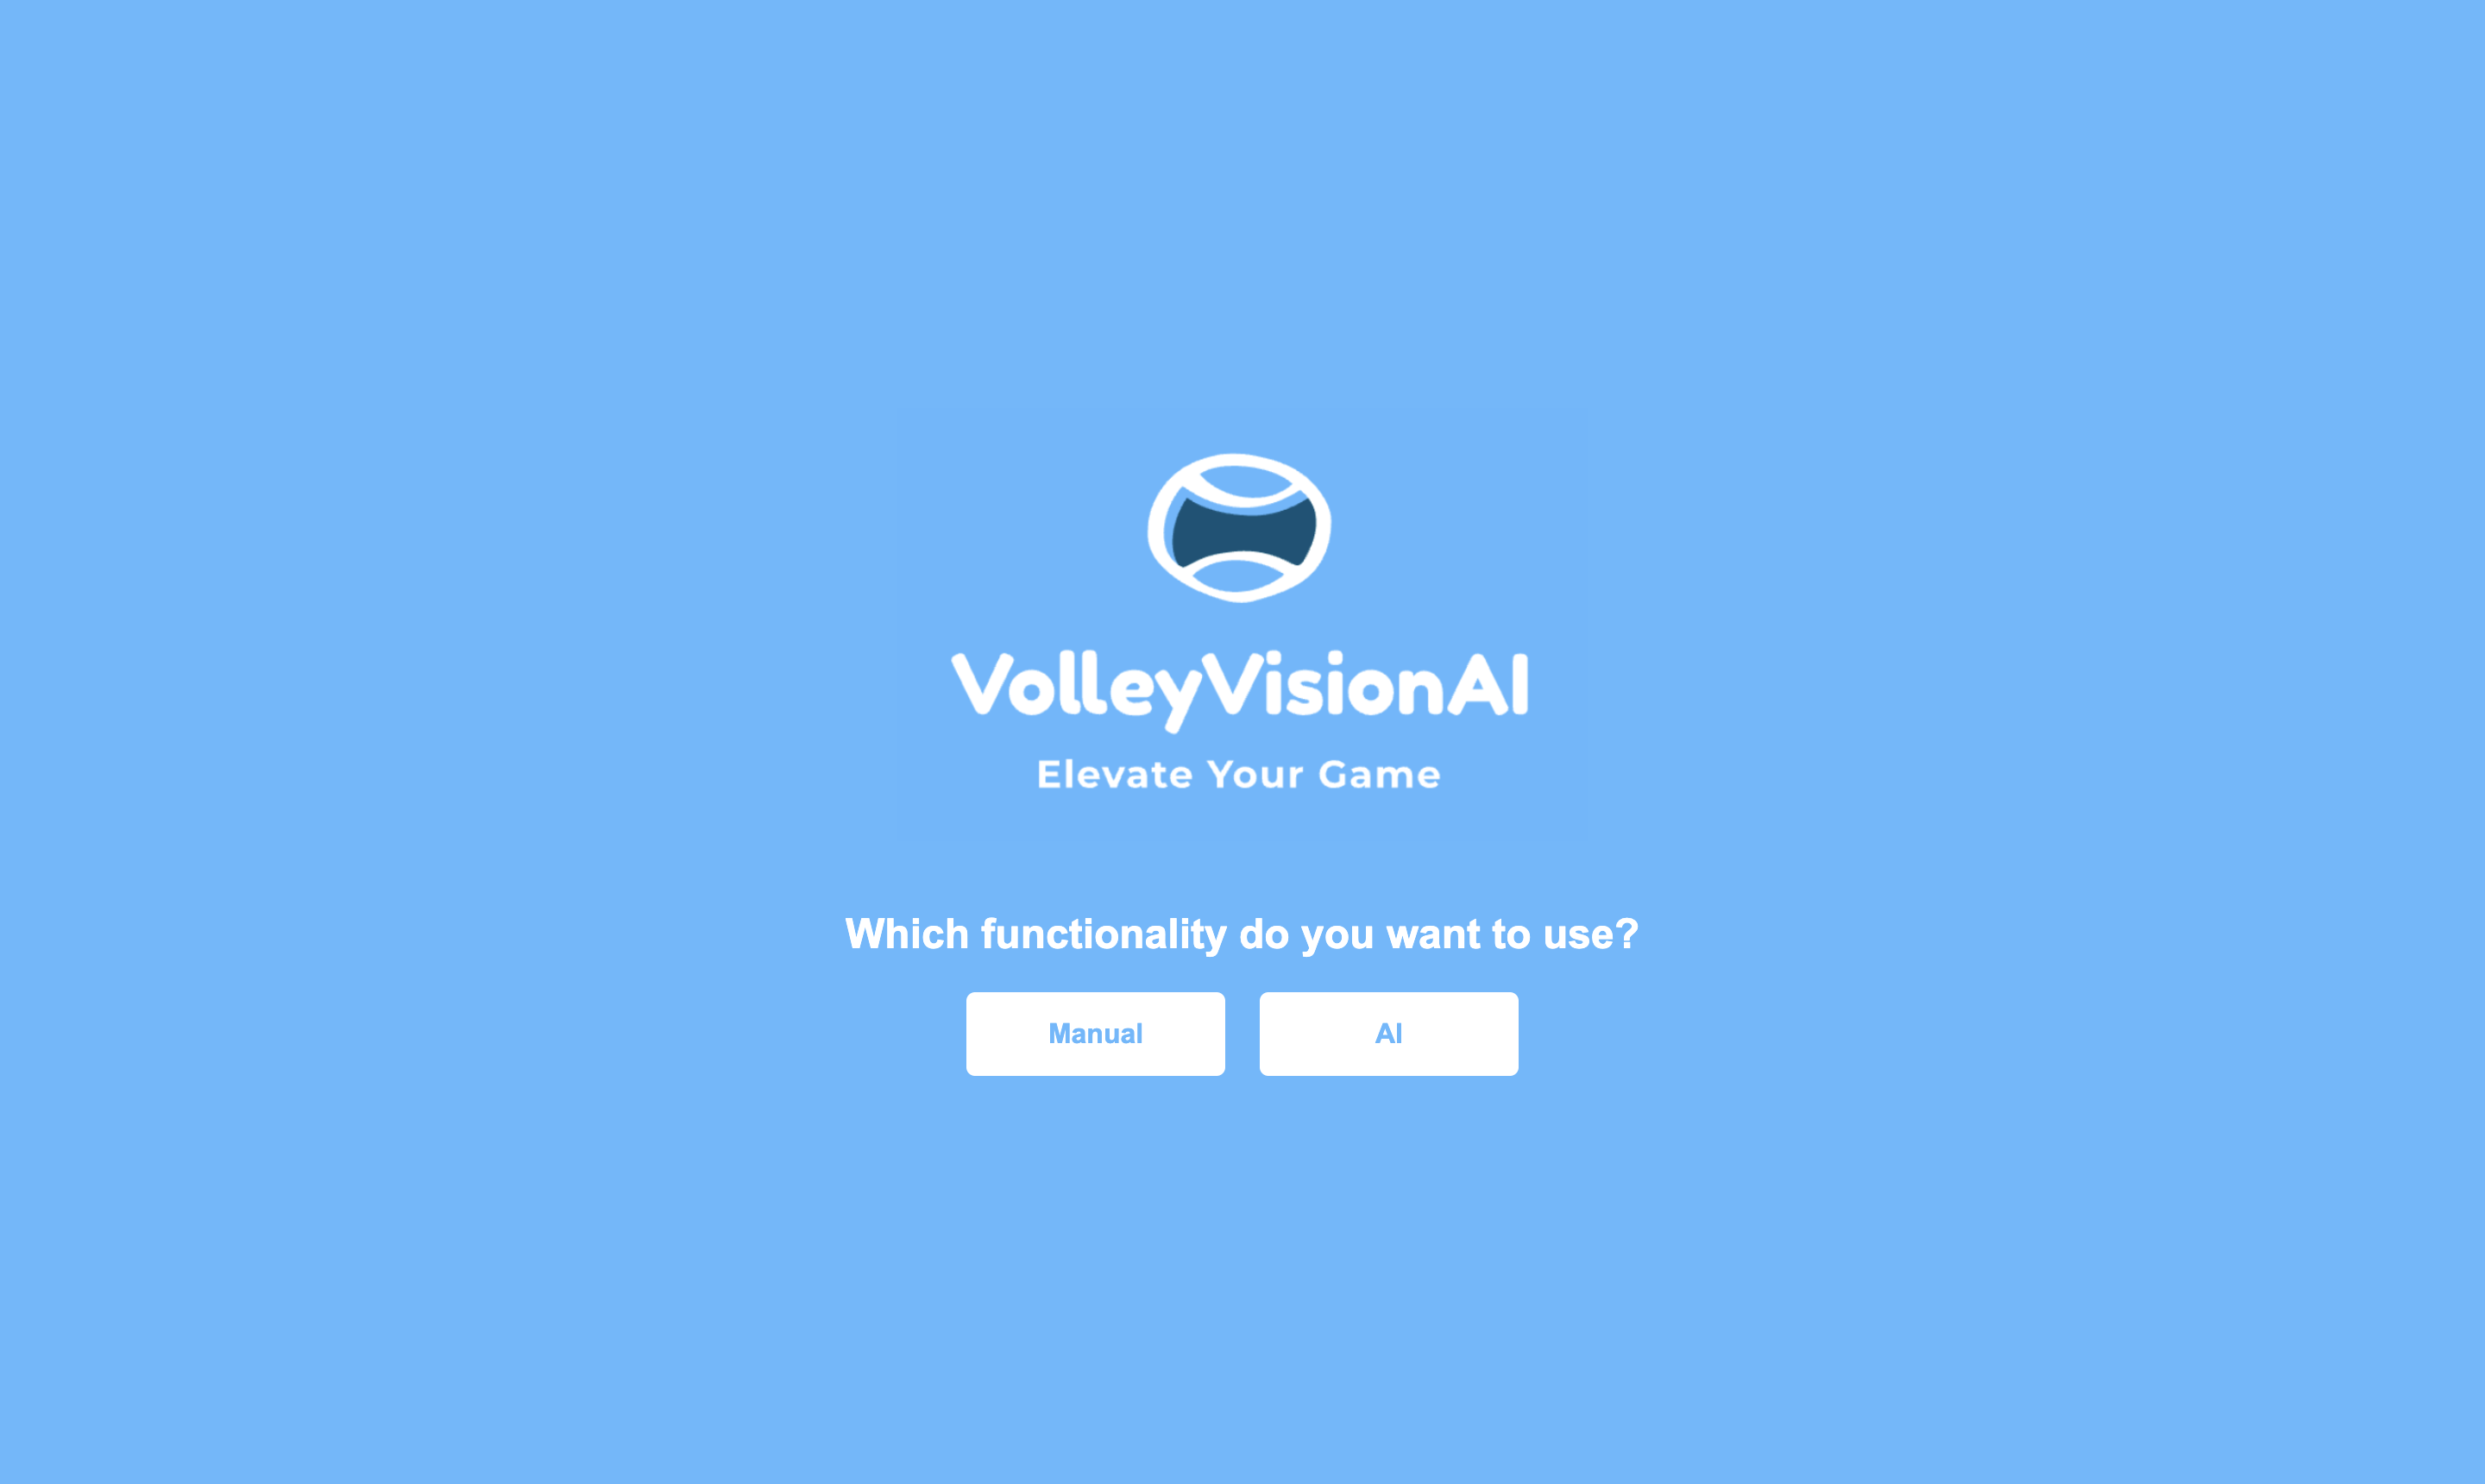
\includegraphics[scale=0.22]{Menu_iniziale.png}}
    \caption{Menu iniziale}
    \label{fig:bot-menu-iniziale}
\end{figure}

\noindent Ciascuna di queste opzioni porta ad una schermata con le relative funzionalità.

\begin{itemize}
    \item \textbf{Manual}: una volta effettuata questa scelta, l'utente dovrà decidere se creare un nuovo progetto o caricare uno già esistente. Nel primo caso l'applicazione chiederà di inserire i nomi degli atleti e le azioni che vuole raccogliere. Essendo la Web App verticale per lo sport della pallavolo, sono già presenti i fondamentali principali come battuta, attacco, difesa, alzata e muro. Questo avviene per facilitare la configurazione, viene comunque permesso di aggiungere ulteriori etichette. Nel caso dell'importazione di un progetto già esistente, la risposta sarà di individuare sul \textit{file-system} il file di un progetto precedentemente esportato. Effettuato questo setup di istruzione, l'applicazione prosegue con la schermata di \textit{Analisi Manuale}.
    
    \item \textbf{AI}: questa modalità richiede di caricare il video da analizzare, specificando il tipo di riconoscimento desiderato, \textit{Ball Tracking} o \textit{Players Recognition}. Dato che questa operazione è delegata al back-end, l'UI mostrerà un messaggio di attesa finchè il video non è stato elaborato, per poi passare alla schermata di \textit{Analisi AI}.
    
\end{itemize}


\noindent In ciascuna delle due opzioni è permesso, in qualsiasi momento, di tornare al menu iniziale attraverso il bottone dedicato.



\subsection{Analisi Manuale}
\label{subsec:funzionalita_manual}

La funzionalità di \textit{Analisi Manuale} consente all'utente di eseguire operazioni manuali come il \textit{tagging} degli eventi, il disegno su video e la creazione di videoclip. La schermata è caratterizzata da quattro elementi principali che permettono all'utente di svolgere le funzionalità descritte in precedenza. Inoltre l'interfaccia usa colori in maniera intelligente per differenziare i vari elementi migliorando la \textit{User Experience} dell'utente finale.

Seguendo una logica di navigazione, le principali funzionalità vengono descritte di seguito.



\newpage

\subsubsection{Add Shortcut}
\begin{wrapfigure}{r}{0.55\textwidth}
    \centering
    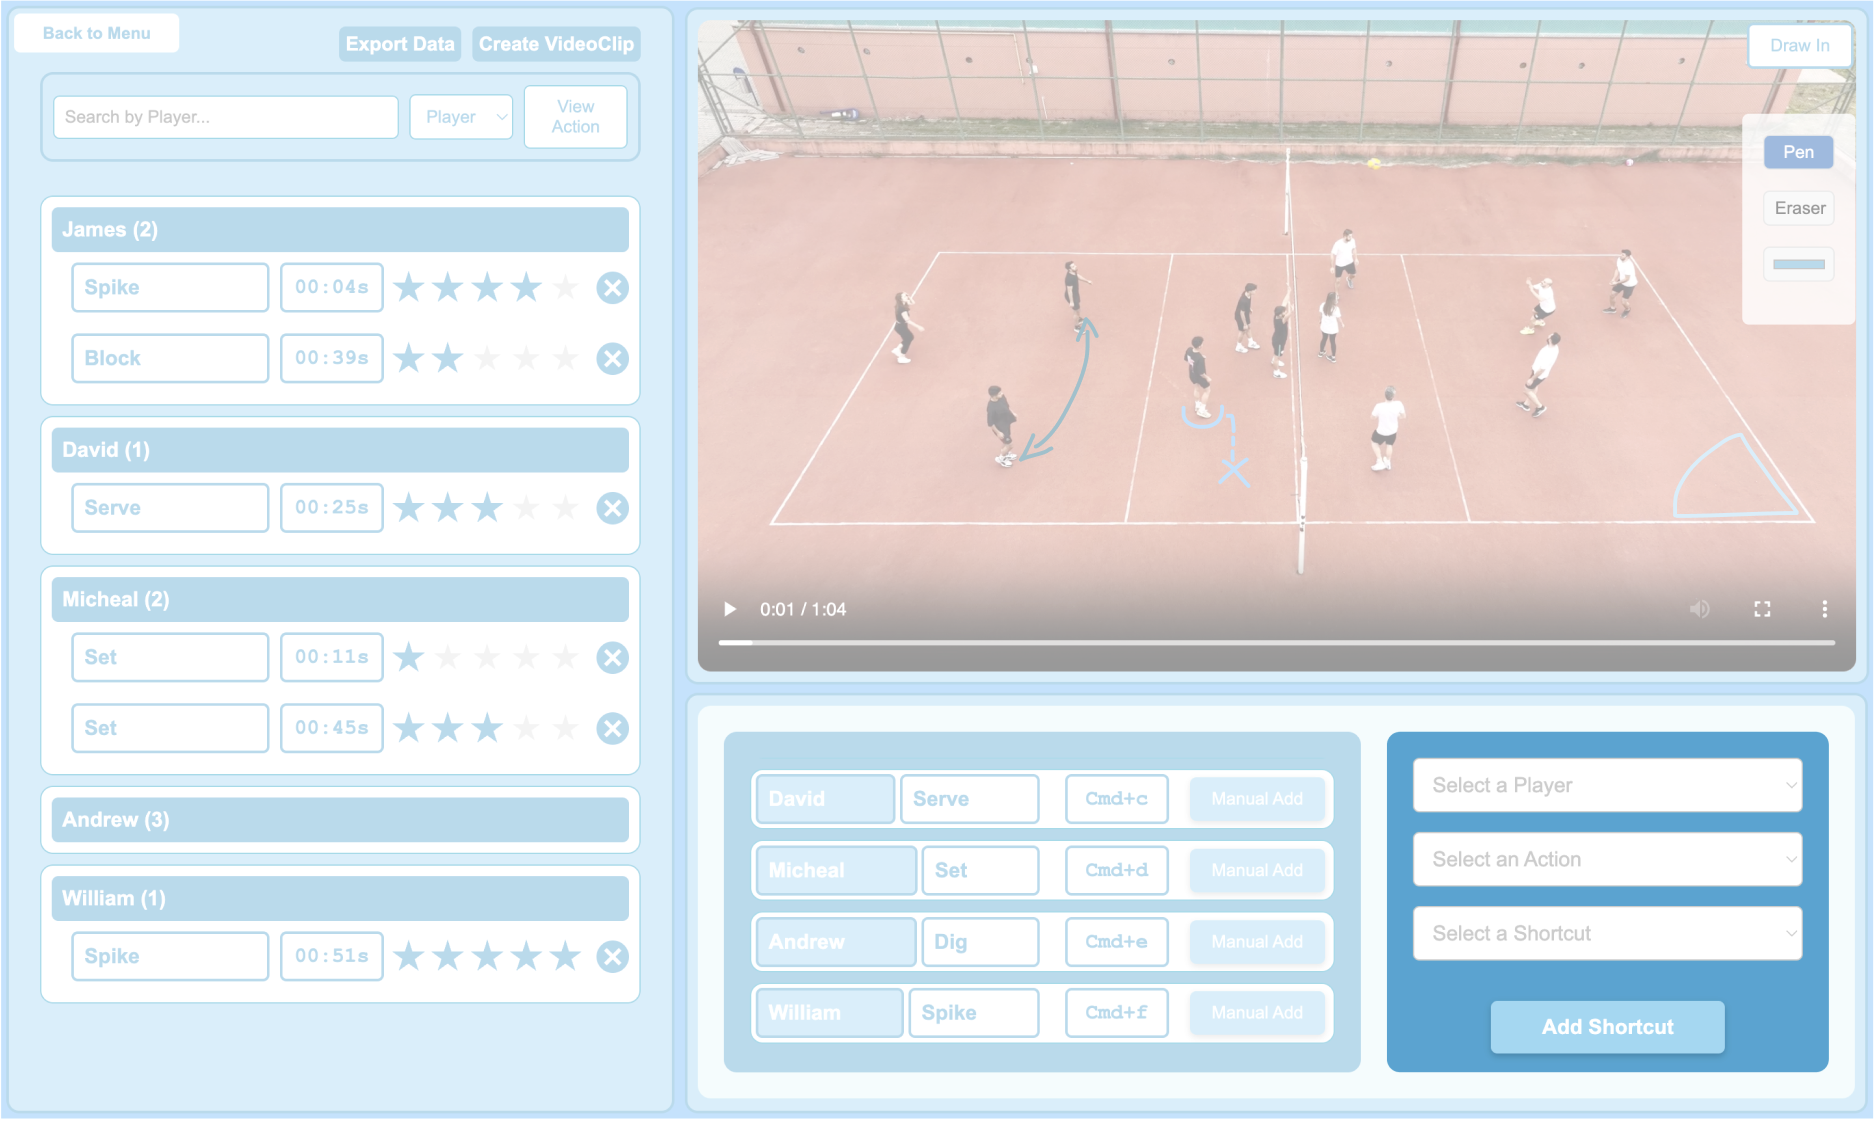
\includegraphics[width=\linewidth]{add_listener.png}
    \captionof{figure}{Add Shortcut}
    \label{fig:add_listener}
\end{wrapfigure}

posto in basso a destra, al di sotto del \textit{VideoPlayer}, si trova un contenitore suddiviso in due componenti di cui l'\textit{Add Shortcut} è quello sulla destra. Questo permette di creare nuovi shortcut personalizzati che servono durante la fase di \textit{Event Tagging}. In particolare è composto da tre menu a tendina che permettono di selezionare l'atleta, l'azione e il comando rapido (shortcut) che si vuole creare. La configurazione dei parametri viene confermata al click sulla voce  "Add Shortcut" sottostante. Naturalmente ogni comando rapido può essere assegnato ad un solo tipo di evento. Se ne viene inserito uno già presente allora l'applicazione rimuove il precedente e lo assegna alla nuova funzionalità scelta.

\subsubsection{Shortcut Summary}
\begin{wrapfigure}{r}{0.55\textwidth}
    \centering
    \vspace{-0.4cm} % Abbassa l'immagine
    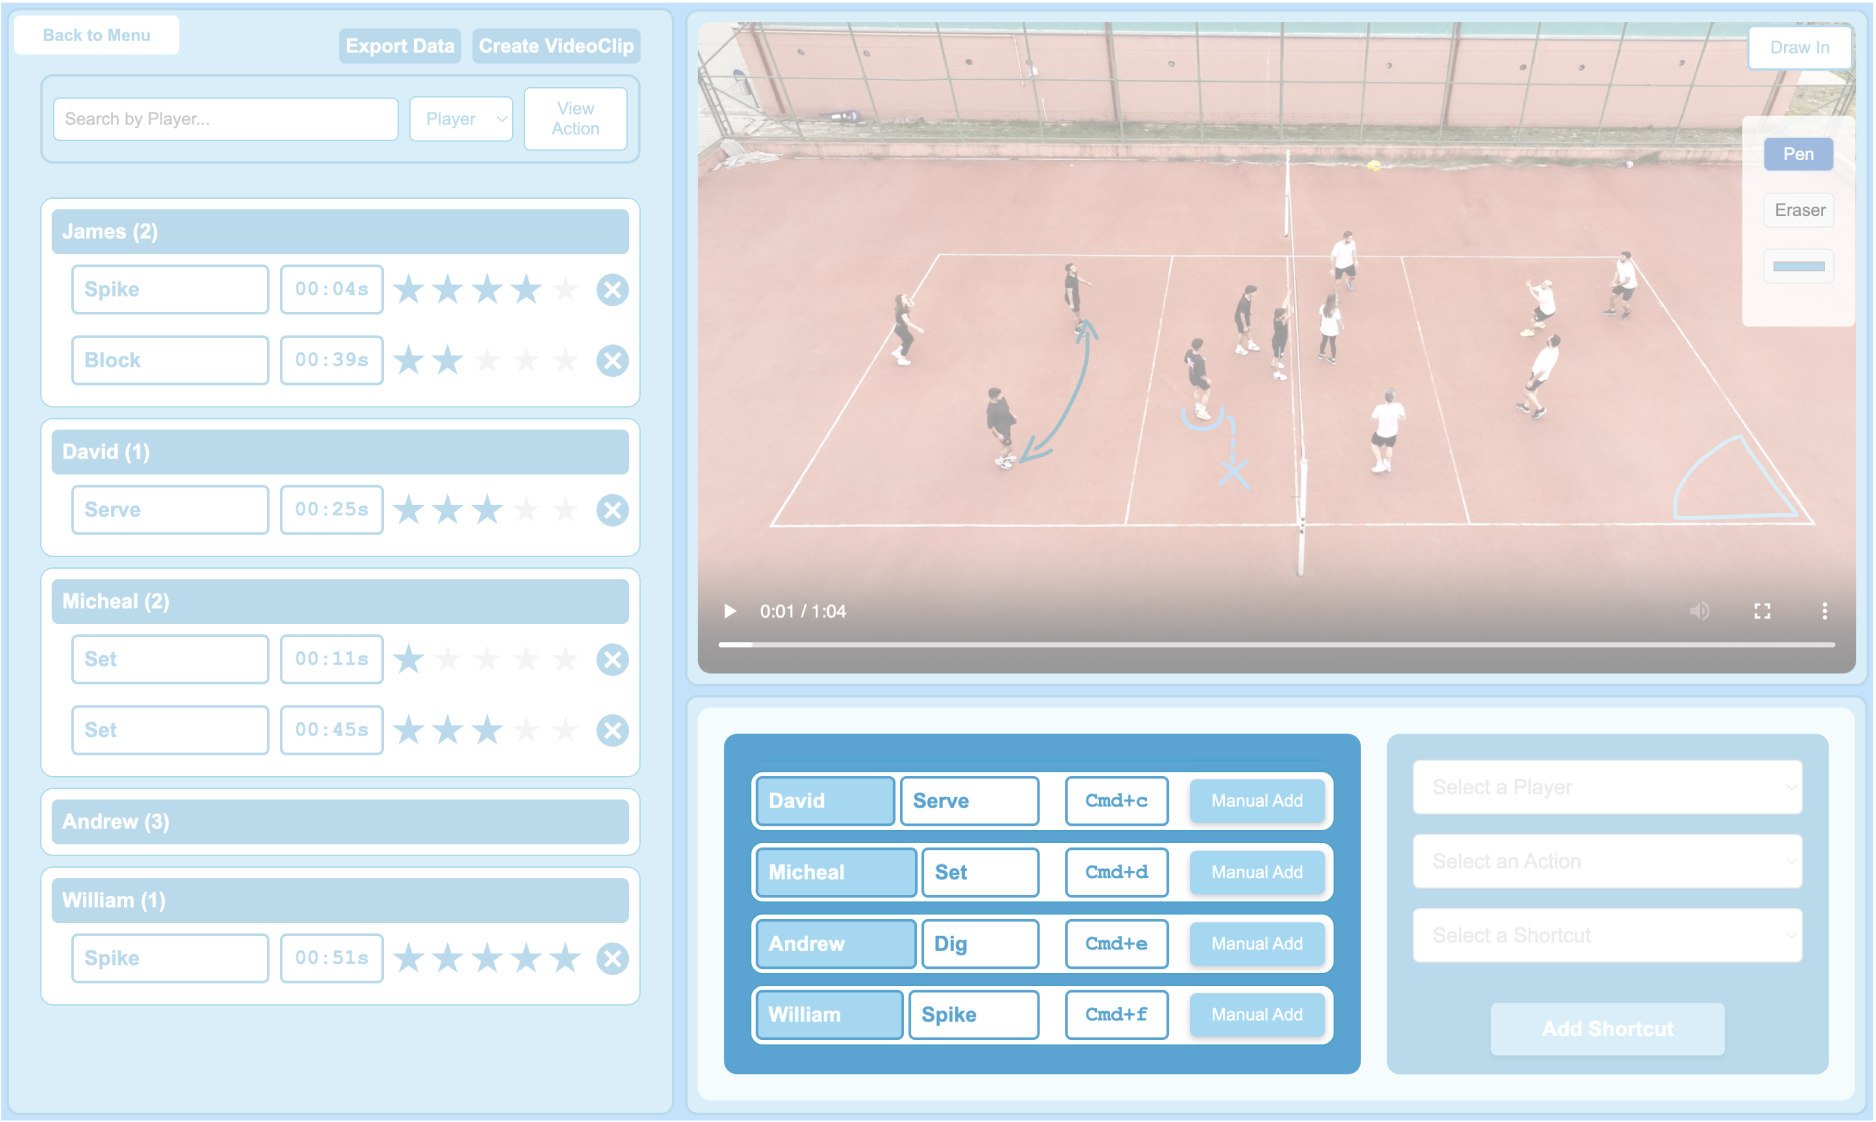
\includegraphics[width=\linewidth]{Summary.png}
    \captionof{figure}{Enabled Shortcut}
    \label{fig:Enabled_shortcut}
\end{wrapfigure}

Creato un qualsiasi shortcut, l'interfaccia presenta, all'interno dello stesso contenitore di \textit{Add Shortcut} ma sulla sua sinistra, il pannello \textit{Shortcut Summary}. La funzione di questo componente permette di tenere traccia degli shortcut creati, rendendoli visualizzabili in una lista che per ognuno ne definisce giocatore, azione e comando rapido. Per migliorare ulteriormente la \textit{User Experience}, ogni shortcut è affiancato da un bottone "Manual Add" che permette ad utenti che non sanno utilizzare gli shortcut da tastiera, di poter comunque utilizzare questa funzionalità dell'app.

\subsubsection{Tagged Events}
\begin{wrapfigure}{r}{0.55\textwidth}
    \centering
    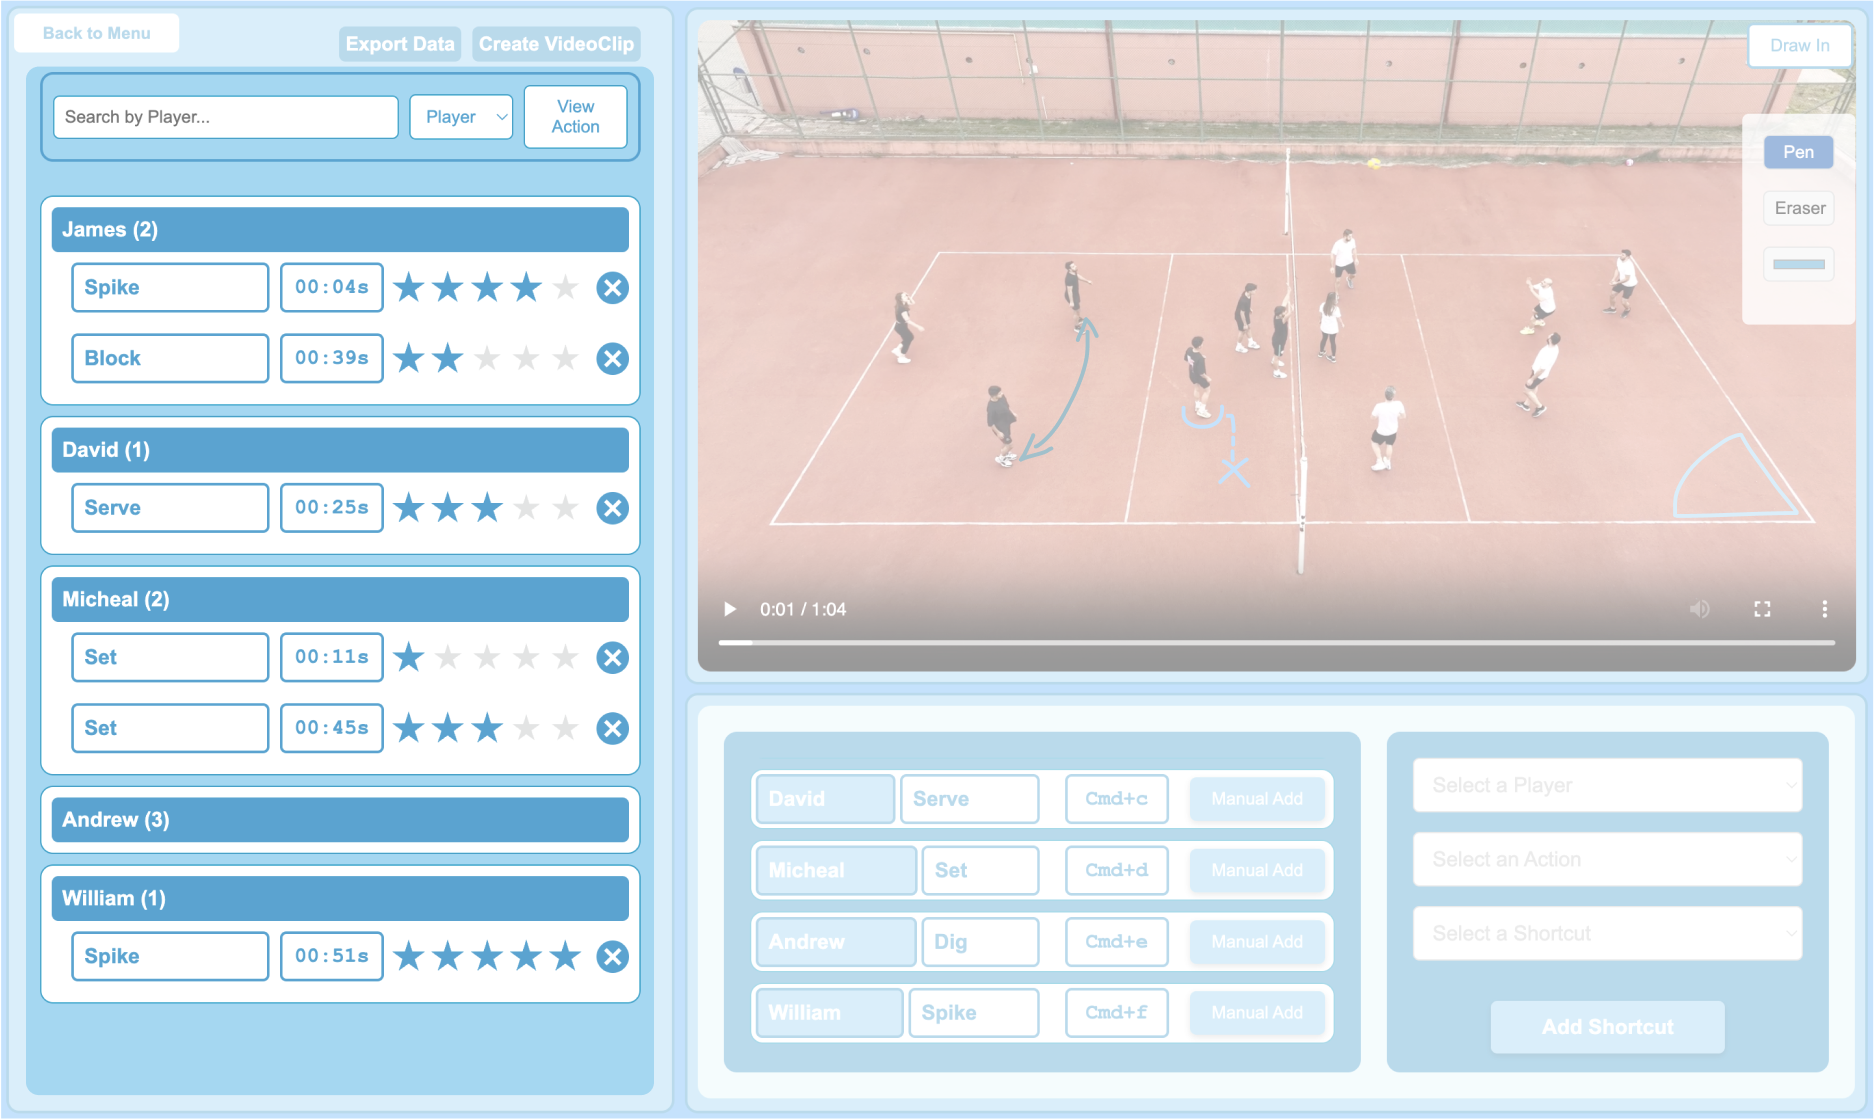
\includegraphics[width=\linewidth]{activated_shortcut.png}
    \captionof{figure}{Tagged Events}
    \label{fig:activated_shortcut}
\end{wrapfigure}

Sulla sezione sinistra dello schermo troviamo uno dei componenti fondamentali della Web App. Una volta che uno shortcut viene attivato, sia tramite comando rapido da tastiera che tramite il bottone "Manual Add" nel componente \textit{Shortcut Summary}, viene visualizzato qui dentro. Il componente è composto da una Search Bar che permette di cercare determinati eventi, selezionando anche se filtrarli in base al giocatore o all'azione. Nell'area sottostante sono invece elencati tutti gli eventi taggati in una lista suddivisa in gruppi. Gli eventi vengono raggruppati in base alla scelta dell'utente, può infatti decidere di visualizzarli in gruppi in base all'azione o in base al giocatore grazie al bottone che cambia tra "View by Action" e "View by Player". L'utente può cambiare questo tipo di visualizzazione in ogni momento. Ad ogni evento taggato corrispondono inoltre altre 2 variabili: il minutaggio e la valutazione. Il primo rappresenta il momento in cui è avvenuto l'evento taggato, dando la possibilità all'utente di cliccarlo per spostare il video a quel preciso istante. Il secondo invece è un componente composto da 5 stelle, inizialmente chiare, che sono utilizzabili dall'utente per dare valutazioni agli eventi taggati. È sempre disponibile, nel caso di uno shortcut attivato per errore, la possibilità di cancellarlo tramite un pulsante X presente accanto ad ognuno.

\subsubsection{Video Player}
\begin{wrapfigure}{r}{0.55\textwidth}
    \centering
    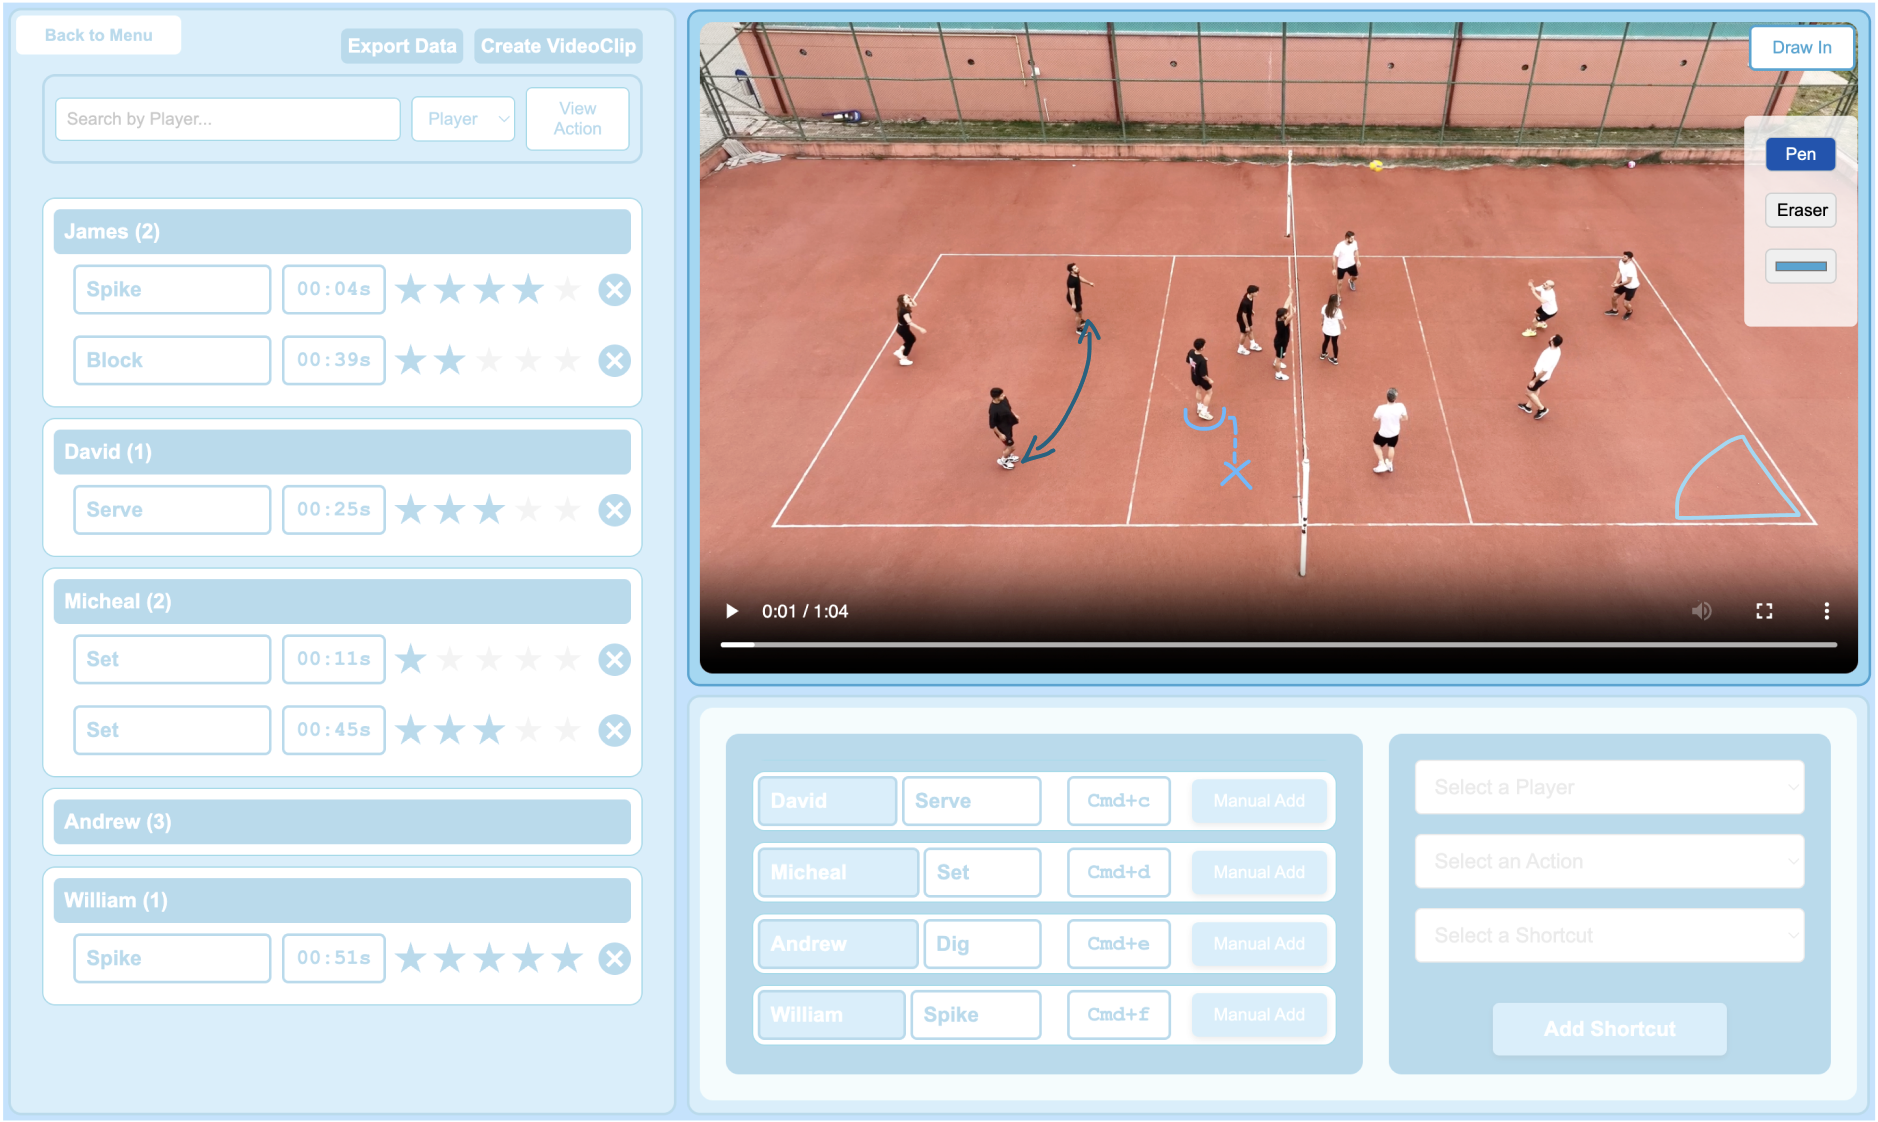
\includegraphics[width=\linewidth]{video_player.png}
    \captionof{figure}{Video Player}
    \label{fig:video_player}
\end{wrapfigure}

In alto a destra, sopra al contenitore di \textit{Shortcut Summary} e \textit{Add Shortcut}, è collocato il componente principale di VolleyVisionAI, ovvero il \textit{Video Player}. Questa sezione mostra all'utente il video caricato permettendo di interagire con esso come un normale \textit{Player Video}, consentendo quindi di controllare la riproduzione, mettere in pausa, avanzare o tornare indietro nel video, e regolare il volume.  Inoltre qui viene implementata la funzionalità di \textit{Drawing} che permette di disegnare sul video. In particolare, tramite il bottone "Draw In" l'utente può attivare la funzionalità di disegno che implementa una dashboard molto semplice.  Quest'ultima permette all'utente di scegliere se usare penna per disegnare o gomma per cancellare. Inoltre è possibile anche scegliere quello che è il colore del tratto, così da aiutare l'utente nel diversificare le sue annotazioni. Ogni volta che l'utente riclicca il pulsante "Draw In" la dashboard e le annotazioni scompariranno, rendendo il video pulito in caso di future annotazioni.

\subsubsection{Export \& Create Videoclip}

Nell'area sovrastante al componente \textit{Tagged Events}, precisamente sopra alla search bar, sono collocati due pulsanti di seguito descritti:
\begin{itemize}
    \item \textbf{Export Project:} consente di esportare il progetto, permettendo all'utente di salvarlo in locale e riutilizzarlo in futuro. In realtà questo bottone non è l'unico che permette di esportare il progetto, infatti se l'utente decide di tornare al menu principale gli verrà richiesto se vuole esportare il progetto prima di abbandonare la pagina. Il progetto viene esportato scaricando sul dispositivo dell'utente un file JSON contenente lo stato dell'app fino a quel momento.
    \item \textbf{Create Videoclip:} consente di creare videoclip in maniera automatica elaborando gli eventi taggati in precedenza. In particolare viene richiesto all'utente di selezionare la durata media delle clip che andranno a comporre il video. Questa scelta viene presentata come una barra scorrevole con estremi 1s e 15s, così da lasciare all'utente margine di scelta. Successivamente l'utente cliccando il bottone "Create Clip" viene messo in attesa finchè il Back-End non ha elaborato il video. Ogni singola clip è caratterizzata dal testo "Giocatore - Azione" di quell'evento taggato. Una volta terminato il processo, la Web App scarica automaticamente il video risultante sul dispositivo dell'utente.
\end{itemize}

\noindent Come scritto in precedenza, infine, è presente il pulsante "Back to Menu" in alto a sinistra che permette all'utente di tornare al menu principale in qualsiasi momento.
% . Quello  di Esportare il progetto, permettendo all'utente di salvare in locale il progetto e poi riutilizzarolo nel futuro. 
% Appena sopra alla Search Bar troviamo 2 pulsanti, uno per esportare il progetto e l'altro per creare un videoclip. Il primo pulsante permette di salvare il progetto corrente come un file JSON, mentre il secondo consente di creare un videoclip a partire dagli eventi taggati. Questo componente è progettato per semplificare il processo di salvataggio e condivisione dei progetti, consentendo all'utente di esportare i risultati in modo rapido e intuitivo.
\pagebreak
\clearpage


\subsection{Analisi AI}
\label{subsec:funzionalita_ai}

L'\textit{Analisi AI}, seppur ancora in stato embrionale, rappresenta la funzionalità più innovativa dell'app. 

Inizialmente una volta scelta questa modalità viene richiesto all'utente di caricare sull'app il video che vuole analizzare e il tipo di analisi AI che vuole applicare.
Una volta inseriti i dati richiesti, tramite il bottone "Apply AI", l'utente viene messo in una schermata d'attesa caratterizzata da una scritta centrale  "Applying Model", in modo tale da far capire all'utente che VolleyVisionAI sta elaborando il risultato.
Una volta che l'output video è stato generato, l'utente viene portato all'effettiva pagina di Analisi AI.
Questa pagina differisce in base al tipo di analisi scelta dall'utente, in particolare se ha scelto di riconoscere la traiettoria della palla o identificare i singoli giocatori.

\subsubsection{Ball Trajectory}
\begin{wrapfigure}{r}{0.55\textwidth}
    \centering
    \vspace{-0.4cm}
    \includegraphics[width=\linewidth]{ball_recognition.png}
    \captionof{figure}{Ball Trajectory}
    \label{fig:ball_trajectory}
\end{wrapfigure}

Questa funzionalità utilizza il modello YOLOv9c per riconoscere la palla. Vengono impostati in particolare 2 parametri: \textit{confidence} e \textit{object-type}. Per questo tipo di analisi impostiamo la confidenza a 0.6 e il tipo di oggetto a "32". Queste specifiche servono rispettivamente per evitare falsi positivi e per specificare al modello che deve riconoscere una palla. Successivamente i risultati di Yolo vengono utilizzati da OpenCV per rappresentare graficamente la traiettoria. In particolare, vengono presi gli ultimi 30 frame della palla e per ognuno di essi viene disegnato un punto giallo. Questo insieme di punti creano visivamente la traiettoria della palla.

\subsubsection{Players Identification}
\begin{wrapfigure}{r}{0.55\textwidth}
    \centering
    \vspace{-0.5cm}
    \includegraphics[width=\linewidth]{player_recognition.png}
    \captionof{figure}{Player Identification}
    \label{fig:player_identification}
\end{wrapfigure}

Questa funzionalità permette all'utente di avere un riconoscimento grafico dei giocatori presenti nel video caricato. In particolare vengono utilizzate delle \textit{Bounding Boxes}, ovvero delle aree colorate che delimitano i giocatori. Ognuna di esse è caratterizzata da un colore diverso e da un identificativo numerico. Il modello YOLOv9c permette di identificare i singoli player assegnando "0" all'\textit{object-type}. Successivamente i risultati vengono elaborati da un algoritmo SORT, definito anche nel paragrafo \ref{sec:implementazione}, che permette di identificare i giocatori utilizzando le loro coordinate, mantenendo così la loro identità.

\vspace{0.5cm}
\noindent L'interfaccia rimane invariata per entrambe le analisi. Presentando una \textit{User Interface} minimalista composta da un player video, una semplice didascalia che indica il tipo di analisi, il bottone per tornare al menu principale e quello per scaricare il video analizzato.
\clearpage








      \newpage
      \chapter{Evaluation}
\label{cha:evaluation}

Nella valutazione della Web App sono stati sviluppati alcuni \textit{usability testing} chiedendo ad un allenatore di pallavolo femminile e ad un giocatore di pallavolo (ovvero due categorie di utenti a cui mi rivolgo) di completare dei task. Da qui si è passati dall'osservazione all'analisi del comportamento all'interno dell'applicazione. Dopo questa prima fase, ho chiesto agli utenti di descrivere quali, secondo la loro prospettiva, sono i punti di forza e di debolezza, chiedendogli quali migliorie apportare. Il risultato delle interviste ha permesso di integrare quanto rilevato dall'analisi con i feedback degli utenti.
% Questa metodologia consiste in sessioni di osservazione diretta, non intrusiva, dell’interazione tra un utente e un servizio digitale. Durante il test vengono assegnati all’utente uno o più task da svolgere; il compito dell’osservatore è quello di analizzare il comportamento nel portarli a termine. Inoltre, ho deciso di utilizzare il metodo \textit{Thinking Aloud}, che consiste nel chiedere all'utente di esprimere ad alta voce i propri pensieri mentre svolge i task assegnati. Questo metodo permette di ottenere informazioni dettagliate sulle azioni compiute dall'utente e sulle motivazioni che lo hanno portato a compierle.



\section{Usability Testing}
Questo l'elenco delle operazioni che è stato chiesto di svolgere:
\begin{itemize}
    \item Accedere alla Web App nella funzionalità \textit{Manual}.
    \item Creare un nuovo progetto, inserendo i dati richiesti a loro scelta.
    \item Abilitare \textit{Shortcut} a loro piacimento.
    \item Testare la funzionalità di \textit{Event Tagging}.
    \item Testare la funzionalità di \textit{Drawing}.
    \item Creare il videoclip degli eventi taggati.
    \item Esportare il progetto.
    \item Ritornare al menu principale.
    \item Utilizzare la funzionalità \textit{AI} per la traiettoria della palla.
\end{itemize}

\noindent Durante i test di usabilità della Web App gli utenti hanno definito l'applicazione intuitiva e di facile utilizzo. Gli utenti hanno particolarmente apprezzato la possibilità di assegnare valutazioni specifiche a ciascuna azione e di creare videoclip personalizzati. Tuttavia, sono emerse alcune problematiche che successivamente sono state implementate al fine di migliorare ulteriormente l'esperienza d'uso. In particolare:

\begin{itemize}
    \item \textbf{Eliminazione dei \textit{Tagged Events}}: inizialmente, la Web App non consentiva agli utenti di eliminare uno \textit{Tagged Event} attivato erroneamente, rendendo l'interfaccia meno flessibile. Per risolvere questo problema, è stato aggiunto un pulsante "X" accanto a ogni shortcut attivato, permettendo così di eliminarlo facilmente. 
    \item \textbf{Pulsante Manuale per fare \textit{Event Tagging}}: dall'analisi del comportamento sull'uso dell'interfaccia è emersa la difficoltà nell'attivare gli \textit{Shortcut} tramite i comandi rapidi da tastiera. Per semplificare ulteriormente l'utilizzo di questa funzione è stato così aggiunto un pulsante "Manual Add" accanto ad ogni \textit{Shortcut} abilitato in modo da consentire di taggare manualmente un evento semplicemente al clic sul relativo pulsante, senza dover ricorrere per forza a combinazioni di tasti. 
    \item \textbf{Feedback della Web App}: sempre dall'analisi del comportamento di riuso dell'applicazione è emerso che, durante la creazione videoclip e applicazione del modello AI, gli utenti percepivano una pagina statica e poco reattiva. Da qui la decisione di fornire un feedback visivo chiaro attraverso l'implementazione di un effetto di sfocatura della pagina con colori chiari, accompagnato da un'icona dinamica al centro dello schermo indicando "Creating Videoclip" o "Applying Model". Questa modifica ha reso maggiormente evidente lo stato dell'operazione in corso, migliorando la percezione di reattività dell'applicazione.
    
\end{itemize}

\section{Feedback e Miglioramenti}
Al termine dei test, sono stati raccolti feedback da questo campione di utenti riguardo a miglioramenti da implementare. I feedback degli allenatori hanno rispecchiato quanto individuato in fase di testing: la necessità di semplificare ulteriormente alcune componenti della Web App sopra descritte. Inoltre, sono emerse richieste aggiuntive da parte di entrambi gli utenti:

\begin{itemize}
    \item \textbf{Analisi \textit{AI}}: Sia l'allenatore che l'atleta hanno espresso l'esigenza di funzionalità \textit{AI} più avanzate. L'allenatore ha suggerito l'introduzione di un sistema di riconoscimento automatico delle azioni per evitare la fase di \textit{Event Tagging} manuale. L'atleta ha proposto invece un analisi AI più verticale ai singoli giocatori. In particolare, ha richiesto di poter visualizzare tutti i momenti in cui un determinato giocatore è protagonista di un azione. Entrambe le proposte sono state accolte e faranno parte degli sviluppi futuri di VolleyVisionAI. 
    \item \textbf{Descrizione Clip Video}: L'atleta ha richiesto di poter avere nel videoclip generato una piccola descrizione per ogni clip, così da rendere ulteriormente più chiari i vari momenti del video. Questo miglioramento è stato implementato e ora il VideoClip generato presenta un Box in alto a destra con la descrizione "Atleta - Azione" relativa al momento visualizzato.
    \item \textbf{Raggruppamento degli \textit{Shortcut}}: In origine, la Web App raggruppava gli eventi taggati esclusivamente per atleta e presentava una barra di ricerca per ricercarne di specifici. Il pallavolista ha suggerito di aggiungere la possibilità di filtrare i \textit{Tagged Event} anche per azione, offrendo una visualizzazione più chiara e ordinata. Questa richiesta è stata implementata con l'aggiunta di un pulsante che consente di alternare tra "View by Action" e "View by Player" nella barra di ricerca, permettendo così una visualizzazione adattabile secondo le preferenze dell'utente.
\end{itemize}

In conclusione, i test di usabilità hanno confermato che VolleyVisionAI è intuitiva e di facile utilizzo, ma hanno anche evidenziato alcune aree di miglioramento. Grazie ai feedback degli utenti, sono state implementate diverse modifiche per rendere l'interfaccia più flessibile e reattiva, migliorando così l'esperienza d'uso complessiva. Inoltre, sono state raccolte richieste di nuove funzionalità che verranno implementate in futuro per arricchire ulteriormente l'offerta della Web App.

      \newpage
      \chapter{Conclusioni}
\label{cha:conclusioni}

In questo capitolo si espone l'analisi degli obiettivi raggiunti e le funzionalità di VolleyVisionAI che ho sviluppato e di come il percorso formativo seguito da studente ha influenzato il processo di progettazione e realizzazione, analizzando lo stato attuale del progetto e concludendo con riflessioni personali sul lavoro svolto e sui risultati ottenuti.

\section{Raggiungimento degli obiettivi}

VolleyVisionAI ha raggiunto gli obiettivi prefissati con successo, completando tutte le fasi necessarie alla realizzazione della Web App. 
In particolare, dopo un'attenta analisi di mercato, ho definito in fase di progettazione i requisiti chiave da implementare. Successivamente ho creato un prototipo dell'interfaccia con Figma, per poi arrivare alla fase di sviluppo vera e propria. Attualmente l'app è funzionante nella sua versione Beta reperibile alla repository GitHub di FBK come VolleyVisionAI \cite{VolleyVisionAI}.






\subsection{Funzionalità della Web App}

Come descritto nel capitolo \ref{cha:analisi_progettazione}, le funzionalità sviluppate permettono all'utente di: 
\begin{itemize}
    \item creare, importare ed esportare progetti di analisi video personali.
    \item creare \textit{shortcut} personalizzati specificando atleta, azione e comando rapido da tastiera.
    \item etichettare eventi specifici durante l'analisi video utilizzando gli shortcut creati in precedenza.
    \item raggruppare gli eventi etichettati per giocatore o azione. 
    \item filtrare gli eventi etichettati tramite una barra di ricerca.
    \item assegnare valutazioni a ciascun evento etichettato.
    \item disegnare e fare annotazioni direttamente sul video tramite una \textit{dashboard} dedicata. 
    \item richiedere all'app di generare un Videoclip contenente le azioni etichettate in precedenza.
    \item utilizzare l'analisi AI per visualizzare la traiettoria della palla durante le fasi di gioco.
    \item utilizzare l'analisi AI per identificare automaticamente i singoli giocatori in campo.
\end{itemize}


\section{Sviluppi Futuri}

VolleyVisionAI è ancora in una fase Beta e sono numerose le aree di sviluppo che potenzialmente possono rendere l'app ancora più completa e funzionale. In particolare, alcuni possibili sviluppi futuri sono descritti dalle seguenti macro-categorie:

\begin{itemize}
    \item \textit{Gestione utenti}: Sarà necessario implementare un sistema di registrazione e autenticazione per consentire agli utenti di avere il proprio account personale sulla piattaforma. Questo permetterà una gestione dei progetti molto più flessibile e dinamica.
    \item \textit{Modelli Computer Vision}: Come specificato nel nome della Web App, la direzione principale è l'implementazione di ulteriori funzionalità AI. In particolare, lo sviluppo di un modello di Computer Vision per il riconoscimento automatico delle azioni, evitando così il processo di \textit{Event Tagging} manuale. 
    \item \textit{Open Source}: In accordo con il tutor aziendale Maurizio Napolitano, è stata presa in considerazione la possibilità di rendere il progetto VolleyVisionAI Open Source. Questo permetterebbe di velocizzare la crescita della Web App e, allo stesso tempo, diffonderla il più possibile.
    \item \textit{Deployment}: Per rendere l'app accessibile a molti più utenti, sarà necessario implementare un sistema di deployment. L'idea è quella di utilizzare inizialmente servizi di cloud hosting e in particolare l'utilizzo di \textit{Vercel} per il Front-End e \textit{Heroku} per il Back-End.
\end{itemize}

\noindent Durante la fase di progettazione tecnica è stata definita un'architettura estremamente scalabile composta da due server: Front-End e Back-End. Anche se il deploy verrà effettuato utilizzando servizi di cloud hosting, a cui verrà delegata in gran parte la gestione delle risorse, le tecnologie utilizzate sono state scelte per garantire un'ottima scalabilità. In particolare \textit{React} e \textit{FastAPI} permettono di creare applicazioni modulari e facilmente estendibili, garantendo un'ottima manutenibilità del codice.

\section{Formazione}

Per la creazione dell'app VolleyVisionAI, lo studio delle tecnologie utilizzate in fase di sviluppo è stato individuale. Il corso universitario di \textit{Ingegneria del Software} mi ha aiutato in fase di analisi e progettazione a definire i requisiti funzionali e non funzionali della Web App. Inoltre, il corso di EyeStudios Academy su \textit{Figma} mi ha permesso di implementare un prototipo interattivo dell'interfaccia utente prima di passare alla fase di sviluppo tecnico. 
Grazie all'esperienza di tirocinio formativo presso la \textit{Fondazione Bruno Kessler} ho potuto approfondire tutte le fasi dello sviluppo web. In particolare, ho acquisito competenze nell'utilizzo di \textit{React} e \textit{JavaScript}, che sono state fondamentali per la realizzazione della Web App. 
Anche il corso di \textit{Introduction to Machine Learning} tenuto dalla professoressa Elisa Ricci mi ha aiutato nel comprendere i concetti principali di questo settore, che poi ho utilizzato durante lo sviluppo della Web App. 

\section{Conclusioni Personali}

Il lavoro svolto per realizzare VolleyVisionAI mi ha fornito un'occasione preziosa per applicare e approfondire le conoscenze acquisite durante il percorso universitario. 
Lo sviluppo di un progetto pratico sarà sicuramente vantaggioso per i futuri impegni lavorativi e rappresenterà un valore aggiunto al proprio portfolio personale.
Questo progetto, insieme all'esperienza di tirocinio, ha consolidato la mia passione per lo sviluppo web e per l'intelligenza artificiale, rendendomi consapevole del percorso formativo che intendo intraprendere in futuro.





      %\input{capitolo4}
      
      
    \endgroup


    % bibliografia in formato bibtex
    %
    % aggiunta del capitolo nell'indice
    \addcontentsline{toc}{chapter}{Bibliografia}
    % stile con ordinamento alfabetico in funzione degli autori
    \bibliographystyle{plain}
    \bibliography{biblio}
    
%%%%%%%%%%%%%%%%%%%%%%%%%%%%%%%%%%%%%%%%%%%%%%%%%%%%%%%%%%%%%%%%%%%%%%%%%%
%%%%%%%%%%%%%%%%%%%%%%%%%%%%%%%%%%%%%%%%%%%%%%%%%%%%%%%%%%%%%%%%%%%%%%%%%%
%% Nota
%%%%%%%%%%%%%%%%%%%%%%%%%%%%%%%%%%%%%%%%%%%%%%%%%%%%%%%%%%%%%%%%%%%%%%%%%%
%% Nella bibliografia devono essere riportati tutte le fonti consultate 
%% per lo svolgimento della tesi. La bibliografia deve essere redatta 
%% in ordine alfabetico sul cognome del primo autore. 
%% 
%% La forma della citazione bibliografica va inserita secondo la fonte utilizzata:
%% 
%% LIBRI
%% Cognome e iniziale del nome autore/autori, la data di edizione, titolo, casa editrice, eventuale numero dell’edizione. 
%% 
%% ARTICOLI DI RIVISTA
%% Cognome e iniziale del nome autore/autori, titolo articolo, titolo rivista, volume, numero, numero di pagine.
%% 
%% ARTICOLI DI CONFERENZA
%% Cognome e iniziale del nome autore/autori (anno), titolo articolo, titolo conferenza, luogo della conferenza (città e paese), date della conferenza, numero di pagine. 
%% 
%% SITOGRAFIA
%% La sitografia contiene un elenco di indirizzi Web consultati e disposti in ordine alfabetico. 
%% E’ necessario:
%%   Copiare la URL (l’indirizzo web) specifica della pagina consultata
%%   Se disponibile, indicare il cognome e nome dell’autore, il titolo ed eventuale sottotitolo del testo
%%   Se disponibile, inserire la data di ultima consultazione della risorsa (gg/mm/aaaa).    
%%%%%%%%%%%%%%%%%%%%%%%%%%%%%%%%%%%%%%%%%%%%%%%%%%%%%%%%%%%%%%%%%%%%%%%%%%
%%%%%%%%%%%%%%%%%%%%%%%%%%%%%%%%%%%%%%%%%%%%%%%%%%%%%%%%%%%%%%%%%%%%%%%%%%
    

    \titleformat{\chapter}
        {\normalfont\Huge\bfseries}{Allegato \thechapter}{1em}{}
    % sezione Allegati - opzionale
    \appendix

\end{document}
